% \documentclass[a4paper]{report}
\documentclass[10pt]{article}
\usepackage[utf8]{inputenc}
\usepackage[spanish]{babel}
\usepackage{amsmath}
\usepackage{amsfonts}
\usepackage{amssymb}
\usepackage{caption}
\usepackage{subcaption}
\usepackage{graphicx}
\usepackage{amsfonts}
\usepackage{fancyhdr}
\usepackage{comment}
\usepackage[shortlabels]{enumitem}
\usepackage[a4paper, top=2.5cm, bottom=2.5cm, left=2.2cm, right=2.2cm]%
{geometry}
\usepackage{listings}
%para que pueda poner tildes en el código
\usepackage{listingsutf8}
\usepackage{multicol}

\usepackage{graphicx}

\title{\LARGE Informática I}
  \author{Guía de Trabajos Prácticos\\[10pt]
    \\\textit{Departamento de Ingeniería Electrónica}
\\Universidad Tecnológica Nacional, Regional Córdoba
}
\date{2020}

% \renewcommand{\@chapapp}{Unidad}
\renewcommand{\thesubsection}{\arabic{subsection}}

\makeatletter
\def\@seccntformat#1{\@ifundefined{#1@cntformat}%
   {\csname the#1\endcsname\quad}%    default
   {\csname #1@cntformat\endcsname}}% enable individual control
\newcommand\section@cntformat{}     % section level
\makeatother

\newcommand{\underspace}
{
  \underline{\hspace{20mm}}
}
\usepackage{xcolor}

\lstdefinestyle{customc}{
    belowcaptionskip=1\baselineskip,
    breaklines=true,
    % frame=L,
    xleftmargin=\parindent,
    language=C,
    showstringspaces=false,
    basicstyle=\large\ttfamily,
    keywordstyle=\bfseries\color{green!40!black},
    commentstyle=\itshape\color{purple!40!black},
    identifierstyle=\color{blue},
    stringstyle=\color{orange},
  }

\lstdefinestyle{pseudocodigo}{
    belowcaptionskip=1\baselineskip,
    breaklines=true,
    % frame=L,
    xleftmargin=\parindent,
    language=pseudo,
    showstringspaces=false,
    basicstyle= \ttfamily,
    keywordstyle=\bfseries\color{black!40!black},
    commentstyle=\itshape\color{purple!40!black},
    % identifierstyle=\color{blue},
    % stringstyle=\color{orange},
  }

% Define Language
\lstdefinelanguage{pseudo}
{
  % list of keywords
  morekeywords={
    mientras,
    hacer,
    para,
    desde,
    hasta,
	si,
	no,
	fin,
	mientras,
    que,
    imprimir,
    leer,
    for
  },
  sensitive=false, % keywords are not case-sensitive
  morecomment=[l]{//}, % l is for line comment
  morecomment=[s]{/*}{*/}, % s is for start and end delimiter
  morestring=[b]" % defines that strings are enclosed in double quotes
}


\begin{document}
  \thispagestyle{empty}

\begin{center}


\includegraphics[scale=.3]{img/utn.eps}

\medskip
UNIVERSIDAD TECNOLÓGICA NACIONAL

Facultad Regional Córdoba

\vspace{3cm}

\textbf{
  \huge
  Informática I
}

\vspace{2cm}

\LARGE{Guía de Trabajos Prácticos}

\vfill

Departamento de Ingeniería Electrónica

\vspace{1cm}

Córdoba, 2023

\vspace{1cm}

Rev 0.3

\end{center}


  \thispagestyle{empty}

\Large{Informática I}\\

\noindent Profesor Titular: Luis E. Toledo\\
Profesor Asociado: Claudio J. Paz\\
Profesora Adjunta: Silvia J. Arias\\

\medskip
\noindent JTP: Nievas Martin\\
JTP: Silvia A. Carrera



  \section{Estructura de una computadora.}

\subsection{Ejercicios:}

\subsubsection{Clasifique los siguientes artículos como hardware o software:}
\begin{itemize}
  \item Procesador
  \item RAM
  \item Zinjai
  \item Preprocesador
  \item Impresora
  \item Explorador de Internet
\end{itemize}

\subsubsection{Responda las siguientes preguntas}
\begin{enumerate}[a)]
  \item Los programas en C normalmente son escritos en un:
  \item ¿Que programa es el encargado de combinar la salida del compilador, con las funciones de bibliotecas para producir el archivo ejecutable?
  \item ¿Cual es el programa que carga en memoria el programa ejecutable, desde el disco?
  \item ¿Como se llama el programa encargado de convertir los programas escritos en lenguajes de alto nivel, al lenguaje 
    de máquina?
  \item ¿Quien es el encargado de colocar un programa en memoria para que pueda ser ejecutado?
  \item ¿Cual es la unidad mínima de información en una computadora?
\end{enumerate}

\subsubsection{Raspberry pi}
La Raspberry Pi puede considerarse como una computadora portátil, un ordenador de placa única u ordenador de placa simple (SBC) de bajo coste desarrollado en el Reino Unido por la Raspberry Pi Foundation, con el objetivo de estimular la enseñanza de informática en las escuelas.
Busque en internet la información necesaria correspondiente al código de colores de una resistencia, y describa en no
mas de una hoja:
\begin{enumerate}[a)]
  \item Cuales son las diferentes versiones de la raspberry pi?
  \item Cuales son sus dimensiones y cuales son sus periféricos?
  \item Que sistema operativos puede utilizar?
  \item Mencionar un proyecto que pueda ser elaborado con esta placa.
\end{enumerate}

\begin{figure}[h!]
\centering
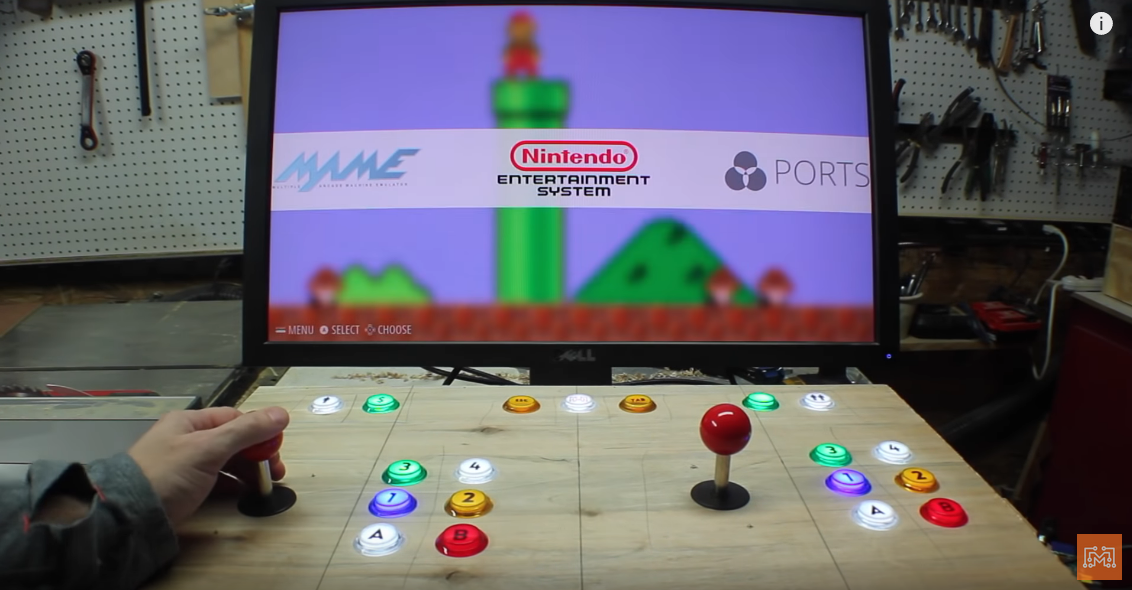
\includegraphics[width=.6\textwidth]{img/retropie.png}
\caption{Consola retropie realizada por ``I Like To Make Stuff''}
\label{fig:retropie}
\end{figure}




  \section{Sistemas de numeración y representación numérica. Aritmética binaria.}
\setcounter{subsection}{2}

\subsubsection{Completar los espacios en blanco:}
\begin{tabular}{ccc}
  Decimal&Binario&Hexadecimal\\
  0&00000000&0x00 \\
  158& &\underspace\\
  145&\underspace &\underspace \\
  \underspace&1010 1110&\underspace \\
  \underspace&0011 1100&\underspace \\
  \underspace&1111 0001&\underspace \\
\end{tabular}

\subsubsection{Suma de números (2.4)}
Realizar las siguientes operaciones, considerando números signados. Expresar el resultado en decimal.
\vspace{10mm}

\begin{tabular}{lc}
$0x3D + 0x40 $&=\underspace\\
$0x3D - 0x20 $&=\underspace\\
$01110110 - 00101101$&=\underspace\\
$00011110 + 01101101$&=\underspace\\

\end{tabular}

\subsubsection{Suma de números (2.4)}
Sin convertir a binario, sumar los siguientes números.

\begin{tabular}{lc}
$0x605C + 0x5 $&=\underspace\\
$0x605C - 0x20 $&=\underspace\\
$0x605C + 32 $&=\underspace\\
$0x60fA - 0x605C $&=\underspace\\
\end{tabular}

\subsubsection{Conversiones}
Realizar las siguientes conversiones:
\begin{itemize}
  \item Convierta el binario 110011010010 en octal y en hexadecimal.
  \item Convierta el número 0xFACE hexadecimal a binaria.
  \item Convierte octal 3016 a binario.
  \item Convierta 0xCAFE hexadecimales a octal.
  \item Convertir binario 1001010 a decimal.
  \item Convertir octal 513 a decimal.
  \item Convierta hexadecimal AFD4 a decimal.
  \item Convierta el decimal 177 a binario, a octal y a hexadecimal.
  \item Calcule la representación binaria del decimal 417. Luego el complemento de 417 y el complemento de dos de 417.
  \item ¿Cuál es el resultado cuando un número y su complemento de dos se suman?
\end{itemize}

% \pagebreak
\subsubsection{ Operaciones Booleanas (2.8)}
Completar los espacios, evaluando las operaciones Booleanas:\\

\begin{tabular}{cc}
  Operación&Resultado\\
  a&[01101010]\\
  b&[11000101]\\
  $\sim$ a&\underspace \\
  $\sim$ b&\underspace \\
  a \& b&\underspace\\
  a $\mid$ b&\underspace\\
  a \^{} b&\underspace\\
\end{tabular}

\subsubsection{Operadores binarios (2.14)}
Realizar las siguientes operaciones binarias, teniendo en cuenta los números anteriormente utilizados.\\

\begin{tabular}{cccc}
  Expresión&Valor&Expresión&Valor\\
  a \& b&\underspace &a \&\& b &\underspace\\
  b $\mid$ b&\underspace& a $\mid\mid$ b &\underspace\\
  $\sim$ a $\mid$ $\sim$ b&\underspace& !a $\mid\mid$ !b &\underspace \\
\end{tabular}


\subsubsection{Desplazamiento de bits (2.16)}
Completar con las representaciones correspondientes para cada desplazamiento.\\

\begin{tabular}{cccccccc}
  \multicolumn{2}{c}{ }& &\multicolumn{2}{c}{Lógico}& &\multicolumn{2}{c}{Lógico}\\
  \multicolumn{2}{c}{a}& &\multicolumn{2}{c}{a$<<$2}& &\multicolumn{2}{c}{a$>>$3}\\
  \cline{1-2}\cline{4-5}\cline{7-8}\\
  Hex&Binario&&Hex&Binario&&Hex&Binario\\
  0xD4&\underspace&&\underspace &\underspace &&\underspace &\underspace\\
  0x64&\underspace&&\underspace &\underspace &&\underspace &\underspace\\
  0xD4&\underspace&&\underspace &\underspace &&\underspace &\underspace\\
  0x44&\underspace&&\underspace &\underspace &&\underspace &\underspace\\
\end{tabular}

\subsubsection{Truncado}
En la siguiente tabla escribir las equivalencias de los números suponiendo que sólo se tienen en cuenta 3 bits\\


\begin{tabular}{cccccccc}
  \multicolumn{2}{c}{Hex} & &\multicolumn{2}{c}{No signado}& &\multicolumn{2}{c}{Complemento a 2}\\
  Original&Truncado&&Original&Truncado&&Original&Truncado\\
  \cline{1-2}\cline{4-5}\cline{7-8}\\
  0x1&1          &&1  &\underspace&&1 & \underspace \\
  0x3&3          &&3  &\underspace&&3 & \underspace \\
  0x5&\underspace&&5  &\underspace&&5 & \underspace \\
  0xC&\underspace&&12 &\underspace&&12& -4\\
  0xE&6          &&14 &\underspace&&14& -2\\
\end{tabular}

\subsubsection{Suma}
Realizar las siguientes sumas utilizando números signados de 4 bits:
\begin{itemize}
  \item $ -8-5= $
  \item $-8+5$
  \item $2+5$
  \item $5+5$
\end{itemize}

% \pagebreak
\subsubsection{Interpretación}
Realizar las siguientes sumas e interpretar el resultado como números signados o no signados:\\

\begin{tabular}{ccccc}
x&y&bin&x+y&x+y\\
&&&(4 bits)&(5bits)\\
11000&11000&\underspace&\underspace&\underspace\\
&&&&\\
10111&01000&\underspace&\underspace&\underspace\\
&&&&\\
00010&00101&\underspace&\underspace&\underspace\\
&&&&\\
01100&00100&\underspace&\underspace&\underspace\\
\end{tabular}



  \section{Introducción al lenguaje C.}
\setcounter{subsection}{3}

\subsubsection{Completar los espacios en blanco} 
\begin{enumerate}
  \item Todo programa en C comienza con la ejecución de la función \underspace.
  \item Todos los cuerpos de las funciones comienzan con \underspace y terminan con \underspace
  \item Todas las declaraciones terminan con \underspace.
  \item La función \underspace de la biblioteca estándar permite mostrar información en la pantalla.
  \item La función \underspace de la biblioteca estándar permite ingresar información desde el teclado.
\end{enumerate}

\subsubsection{Programas}
Escribir un programa en C que resuelva los siguientes problemas (uno por cada enunciado)
\begin{itemize}
  \item Definir las variables, ``unavariable'', ``p345'', ``numero''.
  \item Escribir un mensaje en pantalla, solicitando al usuario ingresar un número entero. Se debe imprimir la
    solicitud, en la cual al final debe incluir dos puntos y dejarse un espacio.
  \item Solicitar al usuario ingresar un número entero y almacenarlo en una variable llamada ``num''.
  \item Imprimir en pantalla el mensaje ``Buen día''.
\end{itemize}

\subsubsection{Ejercicio}
Realizar, para cada enunciado, un programa en C.
\begin{itemize}
  \item Asignar la suma de las variables \textbf{a} y \textbf{b} en \textbf{c}.
  \item Leer 3 números enteros desde el teclado, y almacenarlos en las variables \textbf{p}, \textbf{q} y \textbf{r}.
\end{itemize}

\subsubsection{Verdadero o falso}
Indicar si las siguientes afirmaciones son verdaderas o falsas. Si son falsas, indicar porqué:
\begin{itemize}
  \item La función \textbf{printf} siempre imprime al comienzo de una nueva línea.
  \item Los comentarios son mostrados en la pantalla cuando el programa se está ejecutando.
  \item La secuencia de escape \textbackslash \textbf{n} en la función \textbf{printf}, provoca un salto de línea.
  \item Todas las variables deben definirse antes de ser utilizadas.
  \item El operador de resto (\%) solamente puede ser utilizado en números enteros.
  \item Las variables \textbf{numero} y \textbf{NUmerO} son idénticas.
  \item Los operadores aritméticos \textbf{/,*,+,-,\%} tienen todos el mismo nivel de precedencia.
\end{itemize}

% \subsubsection{Selección}
\subsubsection{Ejercicio 3}
Escribir un algoritmo para calcular la distancia recorrida (m) por un móvil que se desplaza con velocidad constante (m/s) durante un tiempo (s). 
La velocidad y el tiempo serán ingresadas por el usuario.

\subsubsection{Ejercicio 4}
Escribir un algoritmo para obtener el promedio simple de un estudiante a partir de las tres notas parciales.
Las notas serán introducidas una a una por el usuario.

\subsubsection{Ejercicio 5}
En un local se hace un descuento del \%20 cuando la compra supera los \$ 1000. Escribir un algoritmo que calcule el precio a pagar por el cliente
teniendo como dato el valor de la compra.

\subsubsection{Ejercicio 6}
Escribir un algoritmo que determine si un número $n$ tiene tres cifras. El usuario debe ingresar el número $n$.

\subsubsection{Ejercicio 7}
Escribir un algoritmo que solicite ingresar dos números $n1$ y $n2$. Si el primero es mayor que el segundo mostrar la suma de ambos, por otro lado si el segundo es mayor al primero, mostrar el producto entre los números. En caso de que sean iguales imprimir ``Los números son iguales''.


  \section{Introducción a la programación estructurada.}
\setcounter{subsection}{3}

\subsection{Repaso}

\begin{minipage}{0.5\textwidth}
  \textbf{si} \it{condición} \textbf{entonces}\\
  \hspace*{10mm}\it{proceso}\\
  \textbf{fin si}\\
\end{minipage}
\begin{minipage}{0.5\textwidth}
\center
  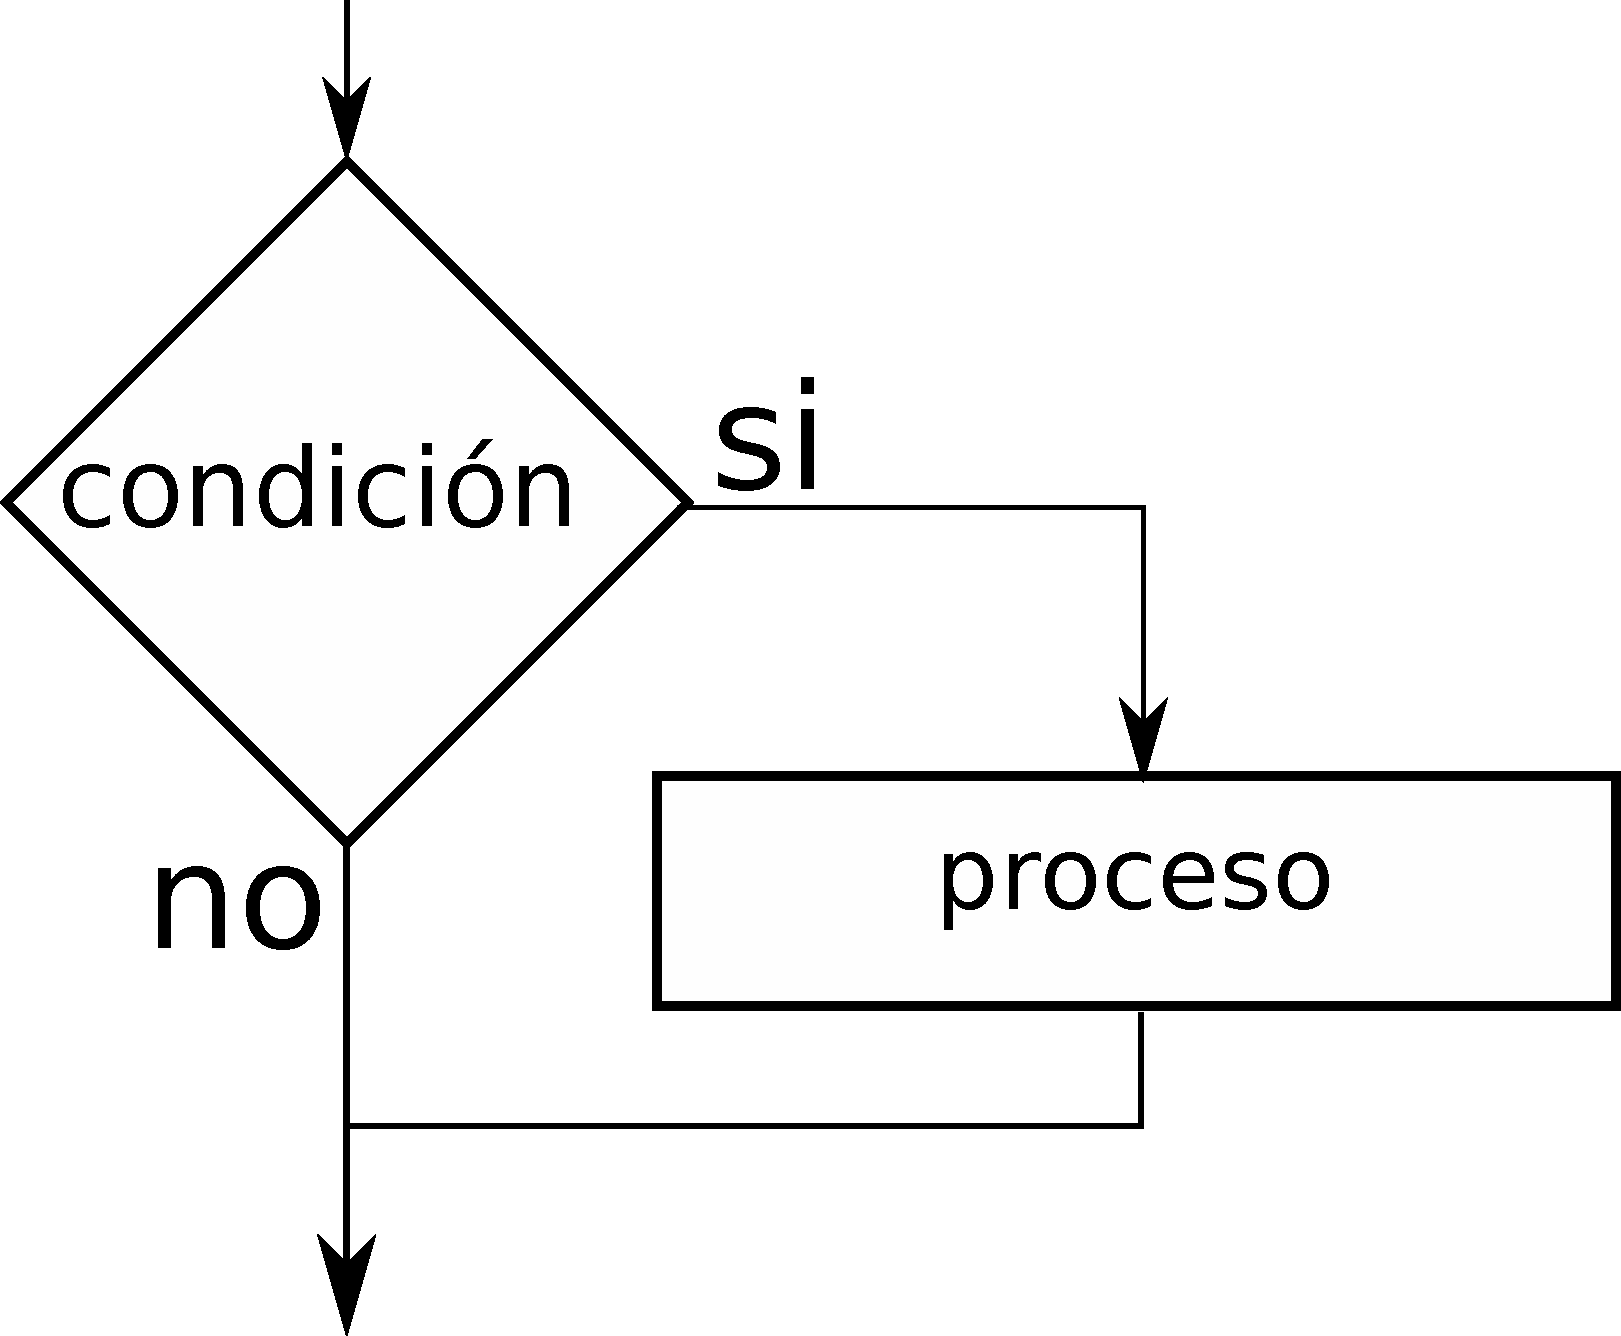
\includegraphics[height=40mm]{img/if.pdf}
\end{minipage}

\vspace{10mm}

\begin{minipage}{0.5\textwidth}
  \textbf{si} \it{condición} \textbf{entonces}\\
  \hspace*{10mm}\it{proceso 1}\\
  \textbf{si no}\\
  \hspace*{10mm}\it{proceso 2}\\
  \textbf{fin si}\\
\end{minipage}
\begin{minipage}{0.5\textwidth}
  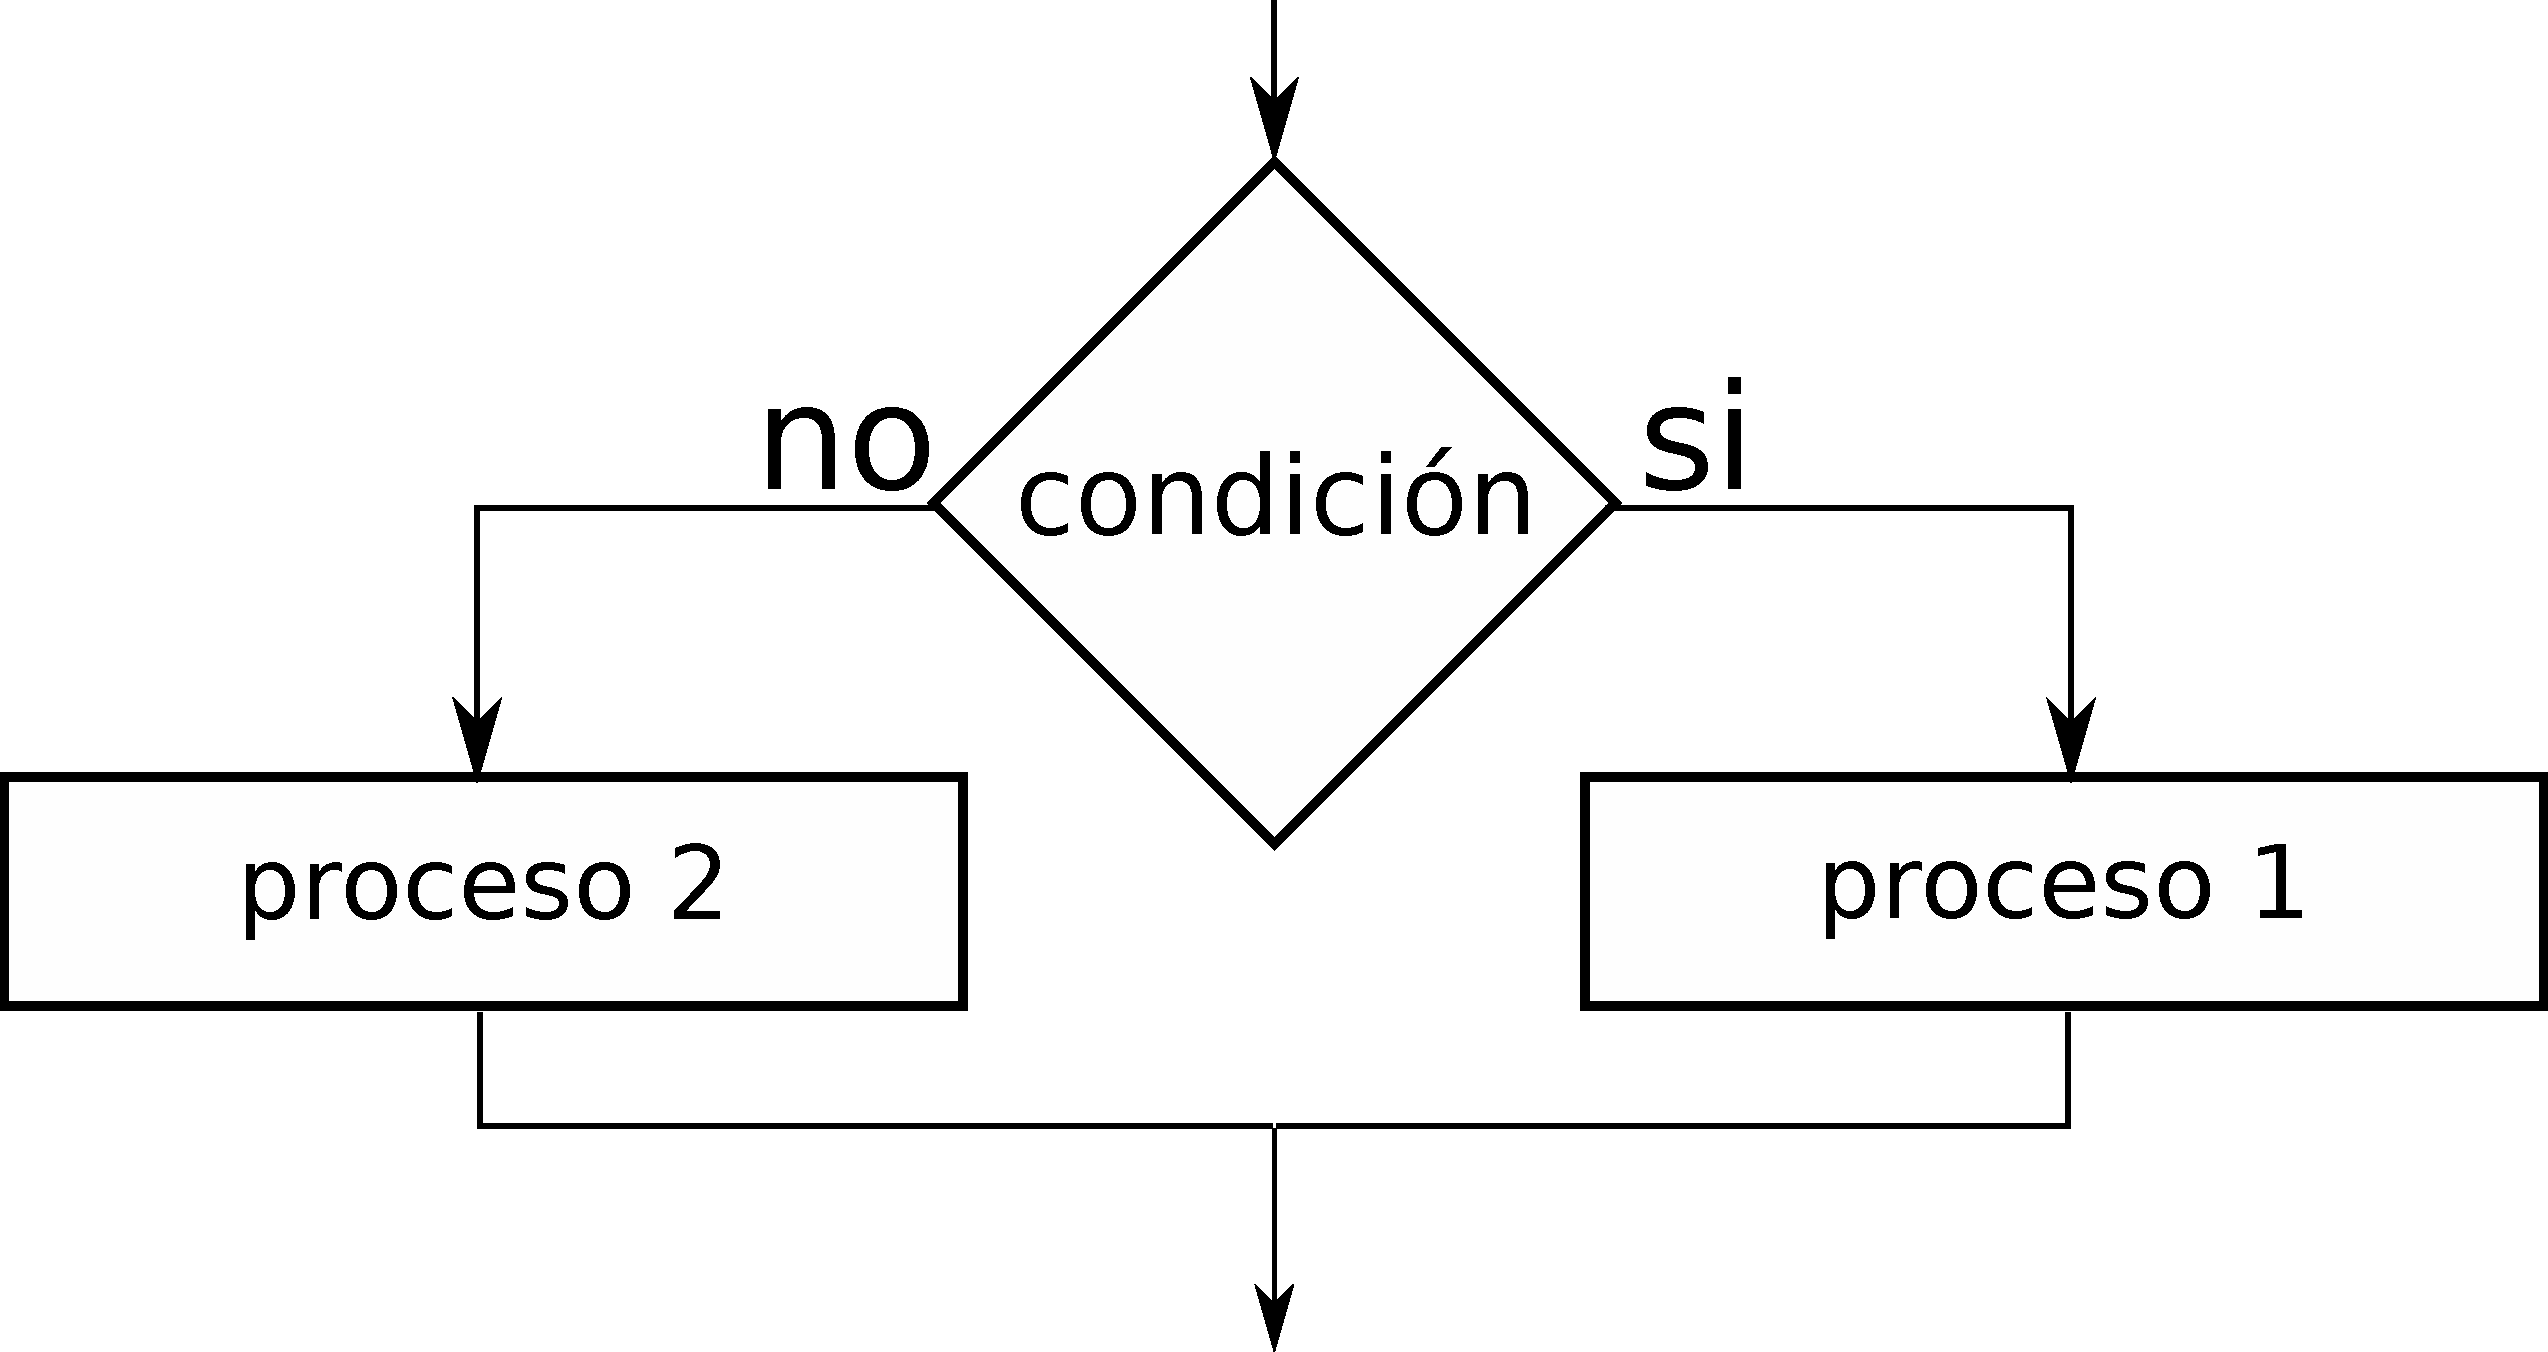
\includegraphics[height=40mm]{img/if_else.pdf}
\end{minipage}

\vspace{10mm}

\begin{minipage}{0.5\textwidth}
  \textbf{mientras} \it{condición} \\
  \hspace*{10mm}\it{proceso}\\
  \textbf{fin mientras}\\
\end{minipage}
\begin{minipage}{0.5\textwidth}
\center
  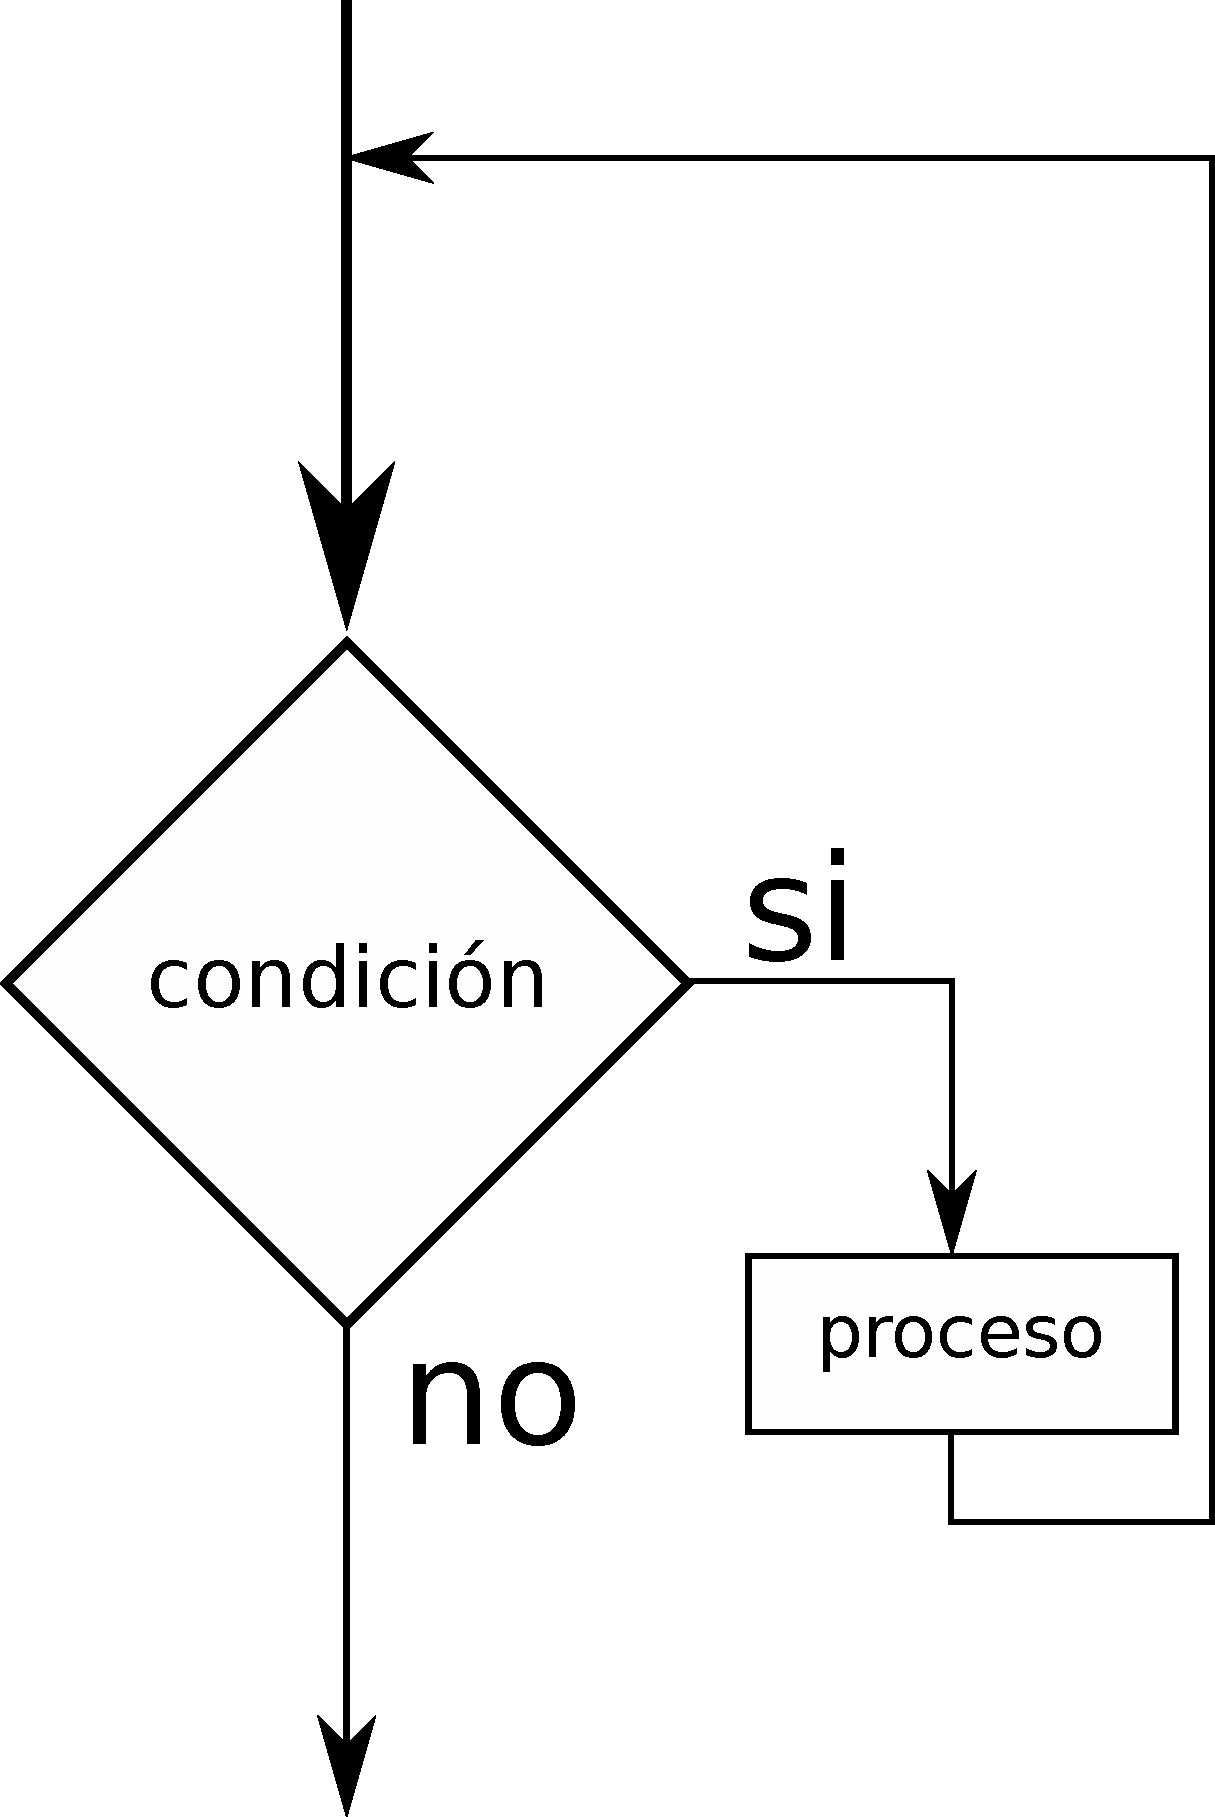
\includegraphics[height=40mm]{img/mientras.pdf}
\end{minipage}

\vspace{10mm}

\begin{minipage}{0.5\textwidth}
  \textbf{hacer} \\
  \hspace*{10mm}\it{proceso}\\
  \textbf{mientras} \it{condición}\\
\end{minipage}
\begin{minipage}{0.5\textwidth}
\center
  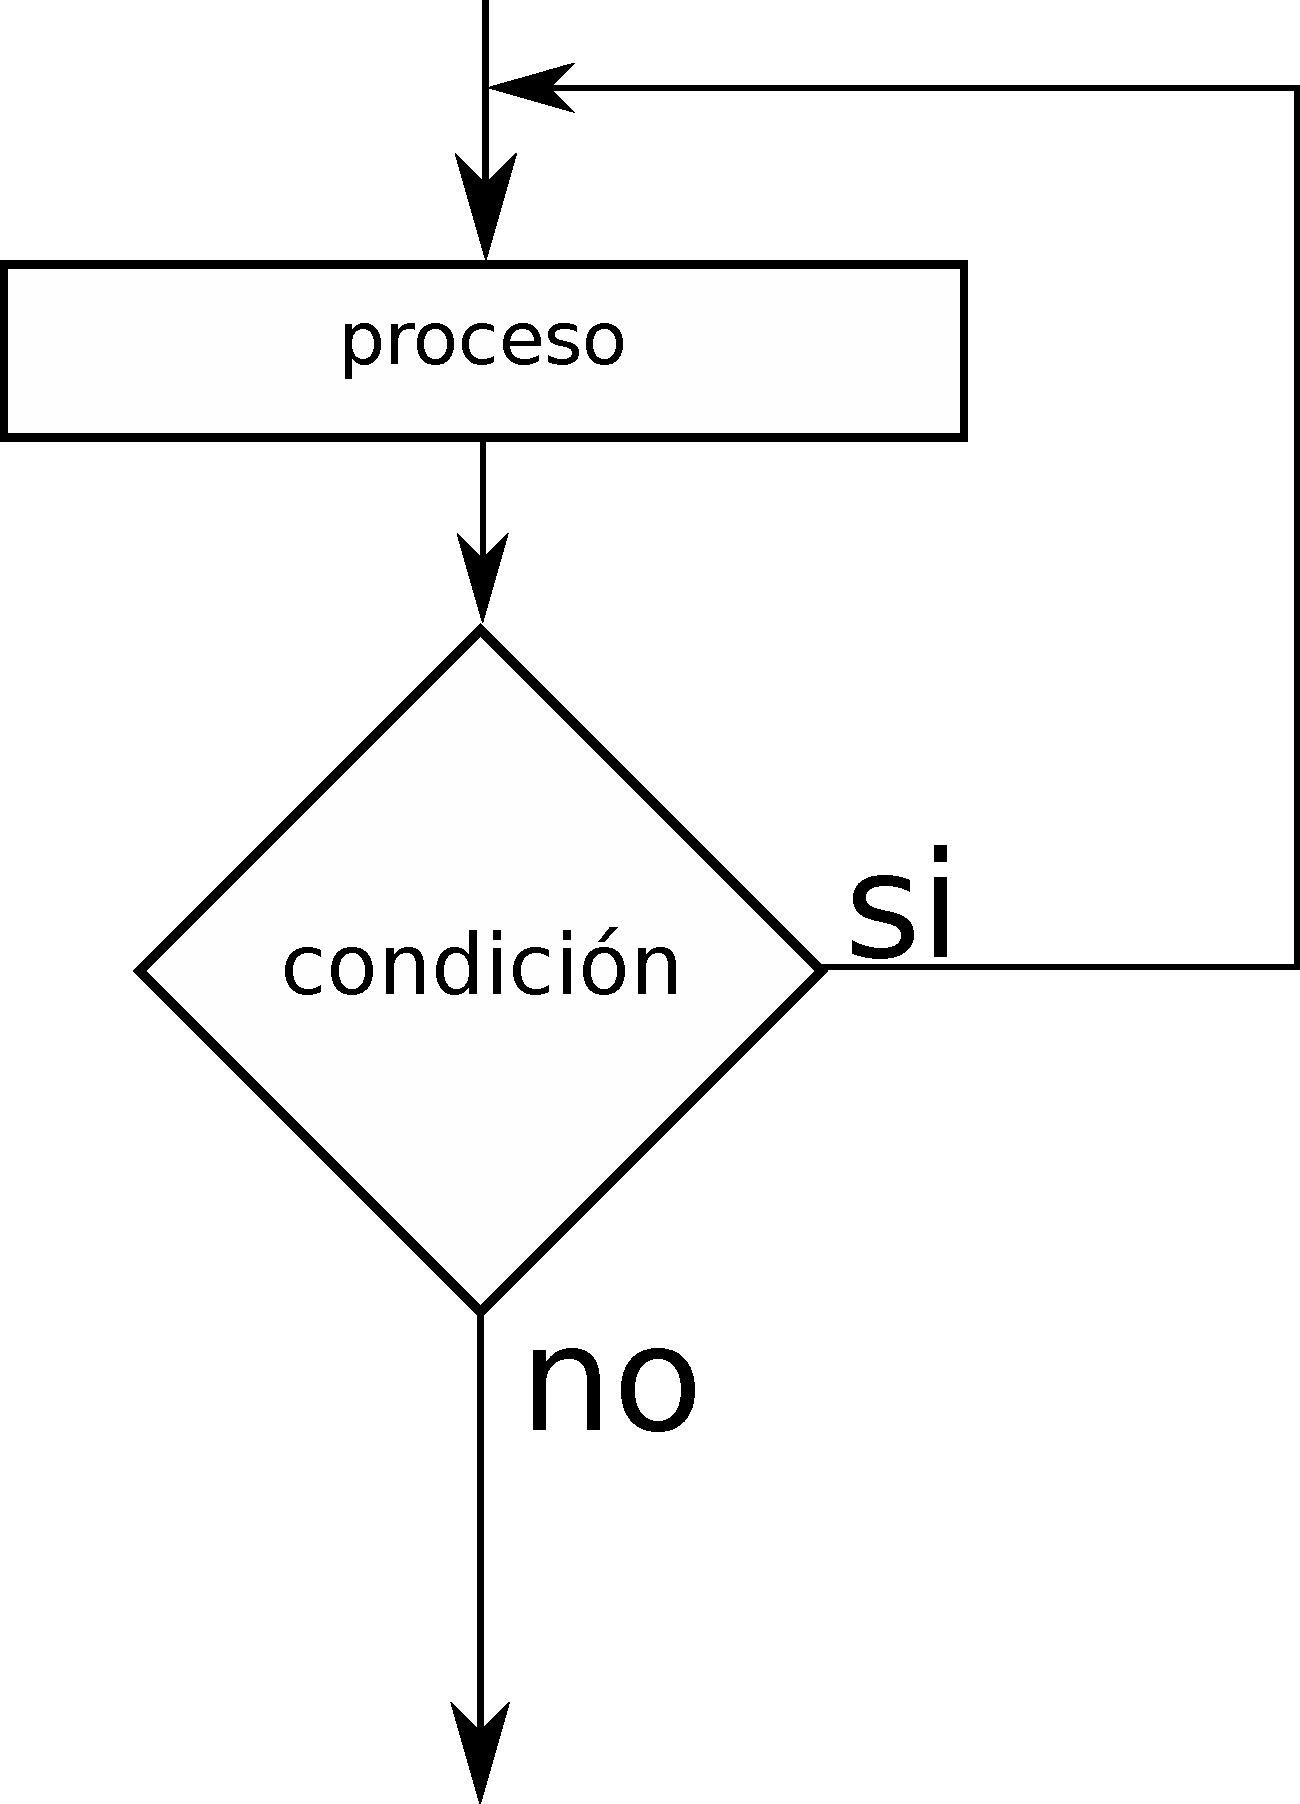
\includegraphics[height=40mm]{img/hacer_mientras.pdf}
\end{minipage}

% \setcounter{subsection}{4}
\subsubsection{Ejercicio}
Realizar un programa que solicite la dimensión en cm de lados de un rectángulo y muestre la superficie del mismo

\subsubsection*{Solución}
\begin{lstlisting}[style=pseudocodigo]
imprimir: Ingrese la longitud del primer lado
leer:lado1
imprimir: Ingrese la longitud del segundo lado
leer: lado2
superficie = lado1 * lado2
imprimir: superficie
\end{lstlisting}

\begin{figure}[h!]
  \centering
  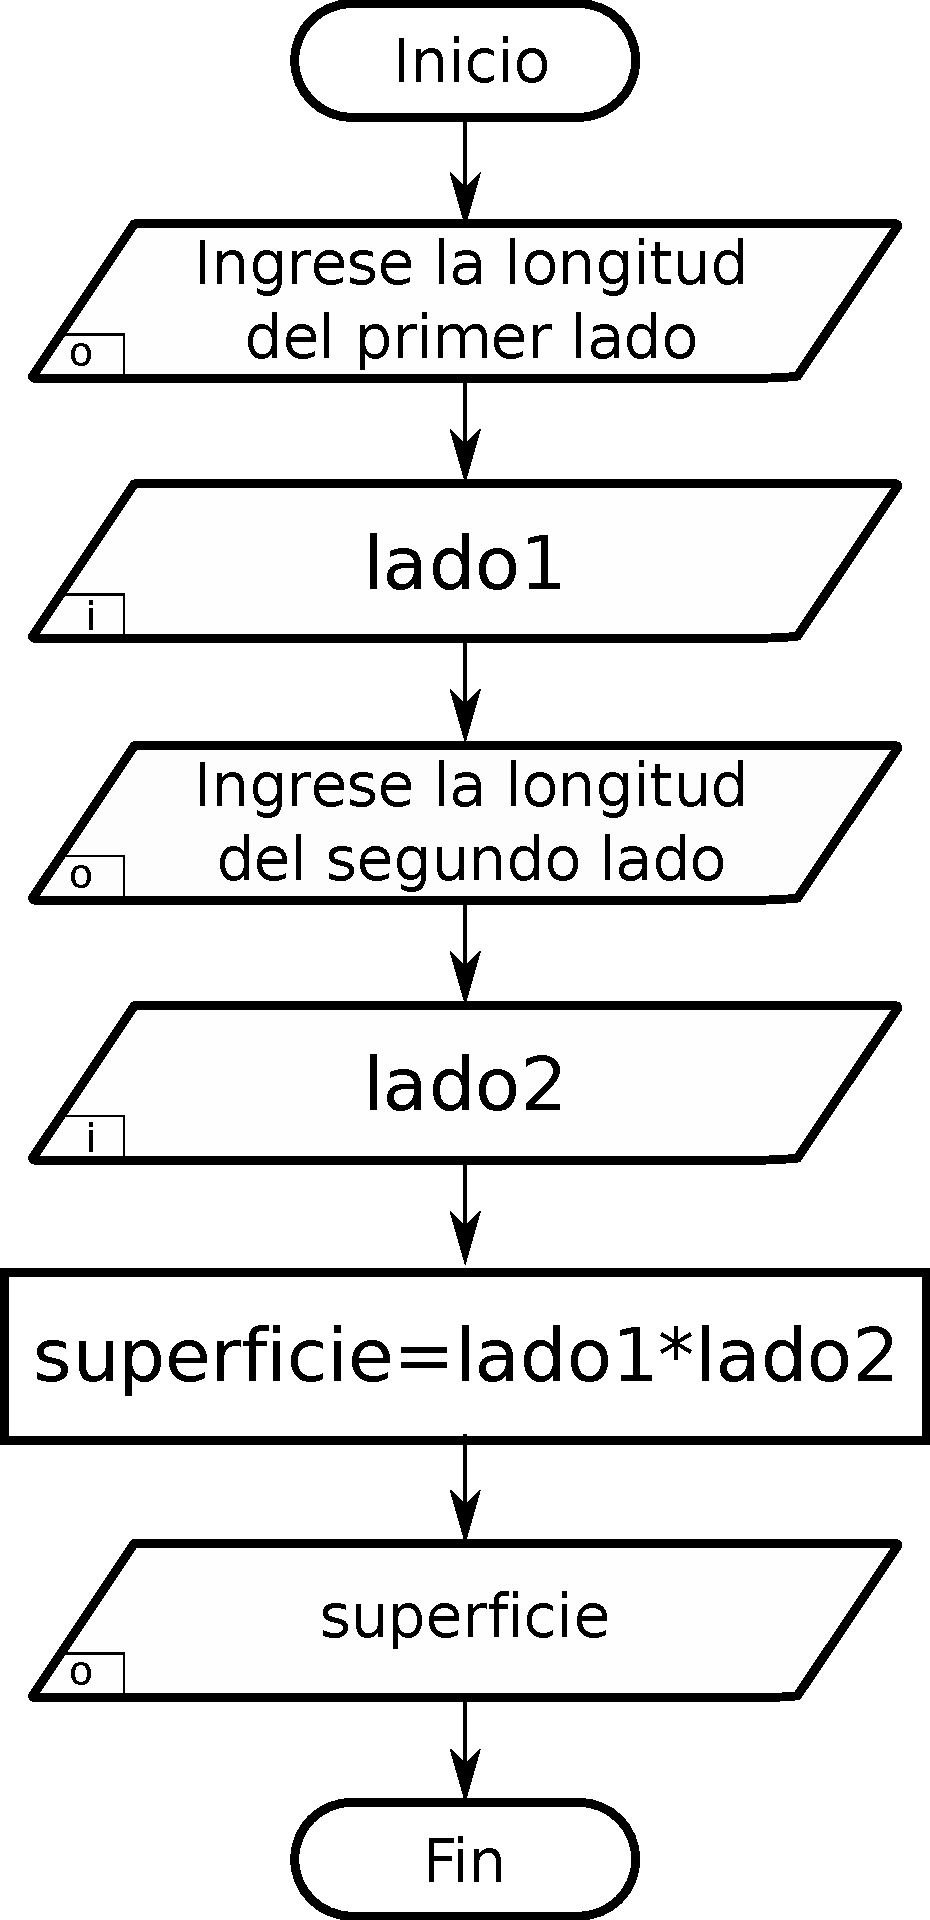
\includegraphics[height=80mm]{./img/ejercicio_1.pdf} 
\end{figure}

\pagebreak

\subsubsection{Ejercicio}
Escribir un algoritmo que solicite la edad de dos hermanos, muestre un mensaje indicando el mayor y su diferencia.

\subsubsection*{Solución}
\begin{lstlisting}[style=pseudocodigo]
imprimir: Ingrese la primera edad
leer:edad1
imprimir: Ingrese la segunda edad
leer: edad2
si edad1 > edad2 entonces
  imprimir: El primero es el mayor
si no
  imprimir: El segundo es el mayor
imprimir: diferencia
\end{lstlisting}

\begin{figure}[h!]
  \centering
  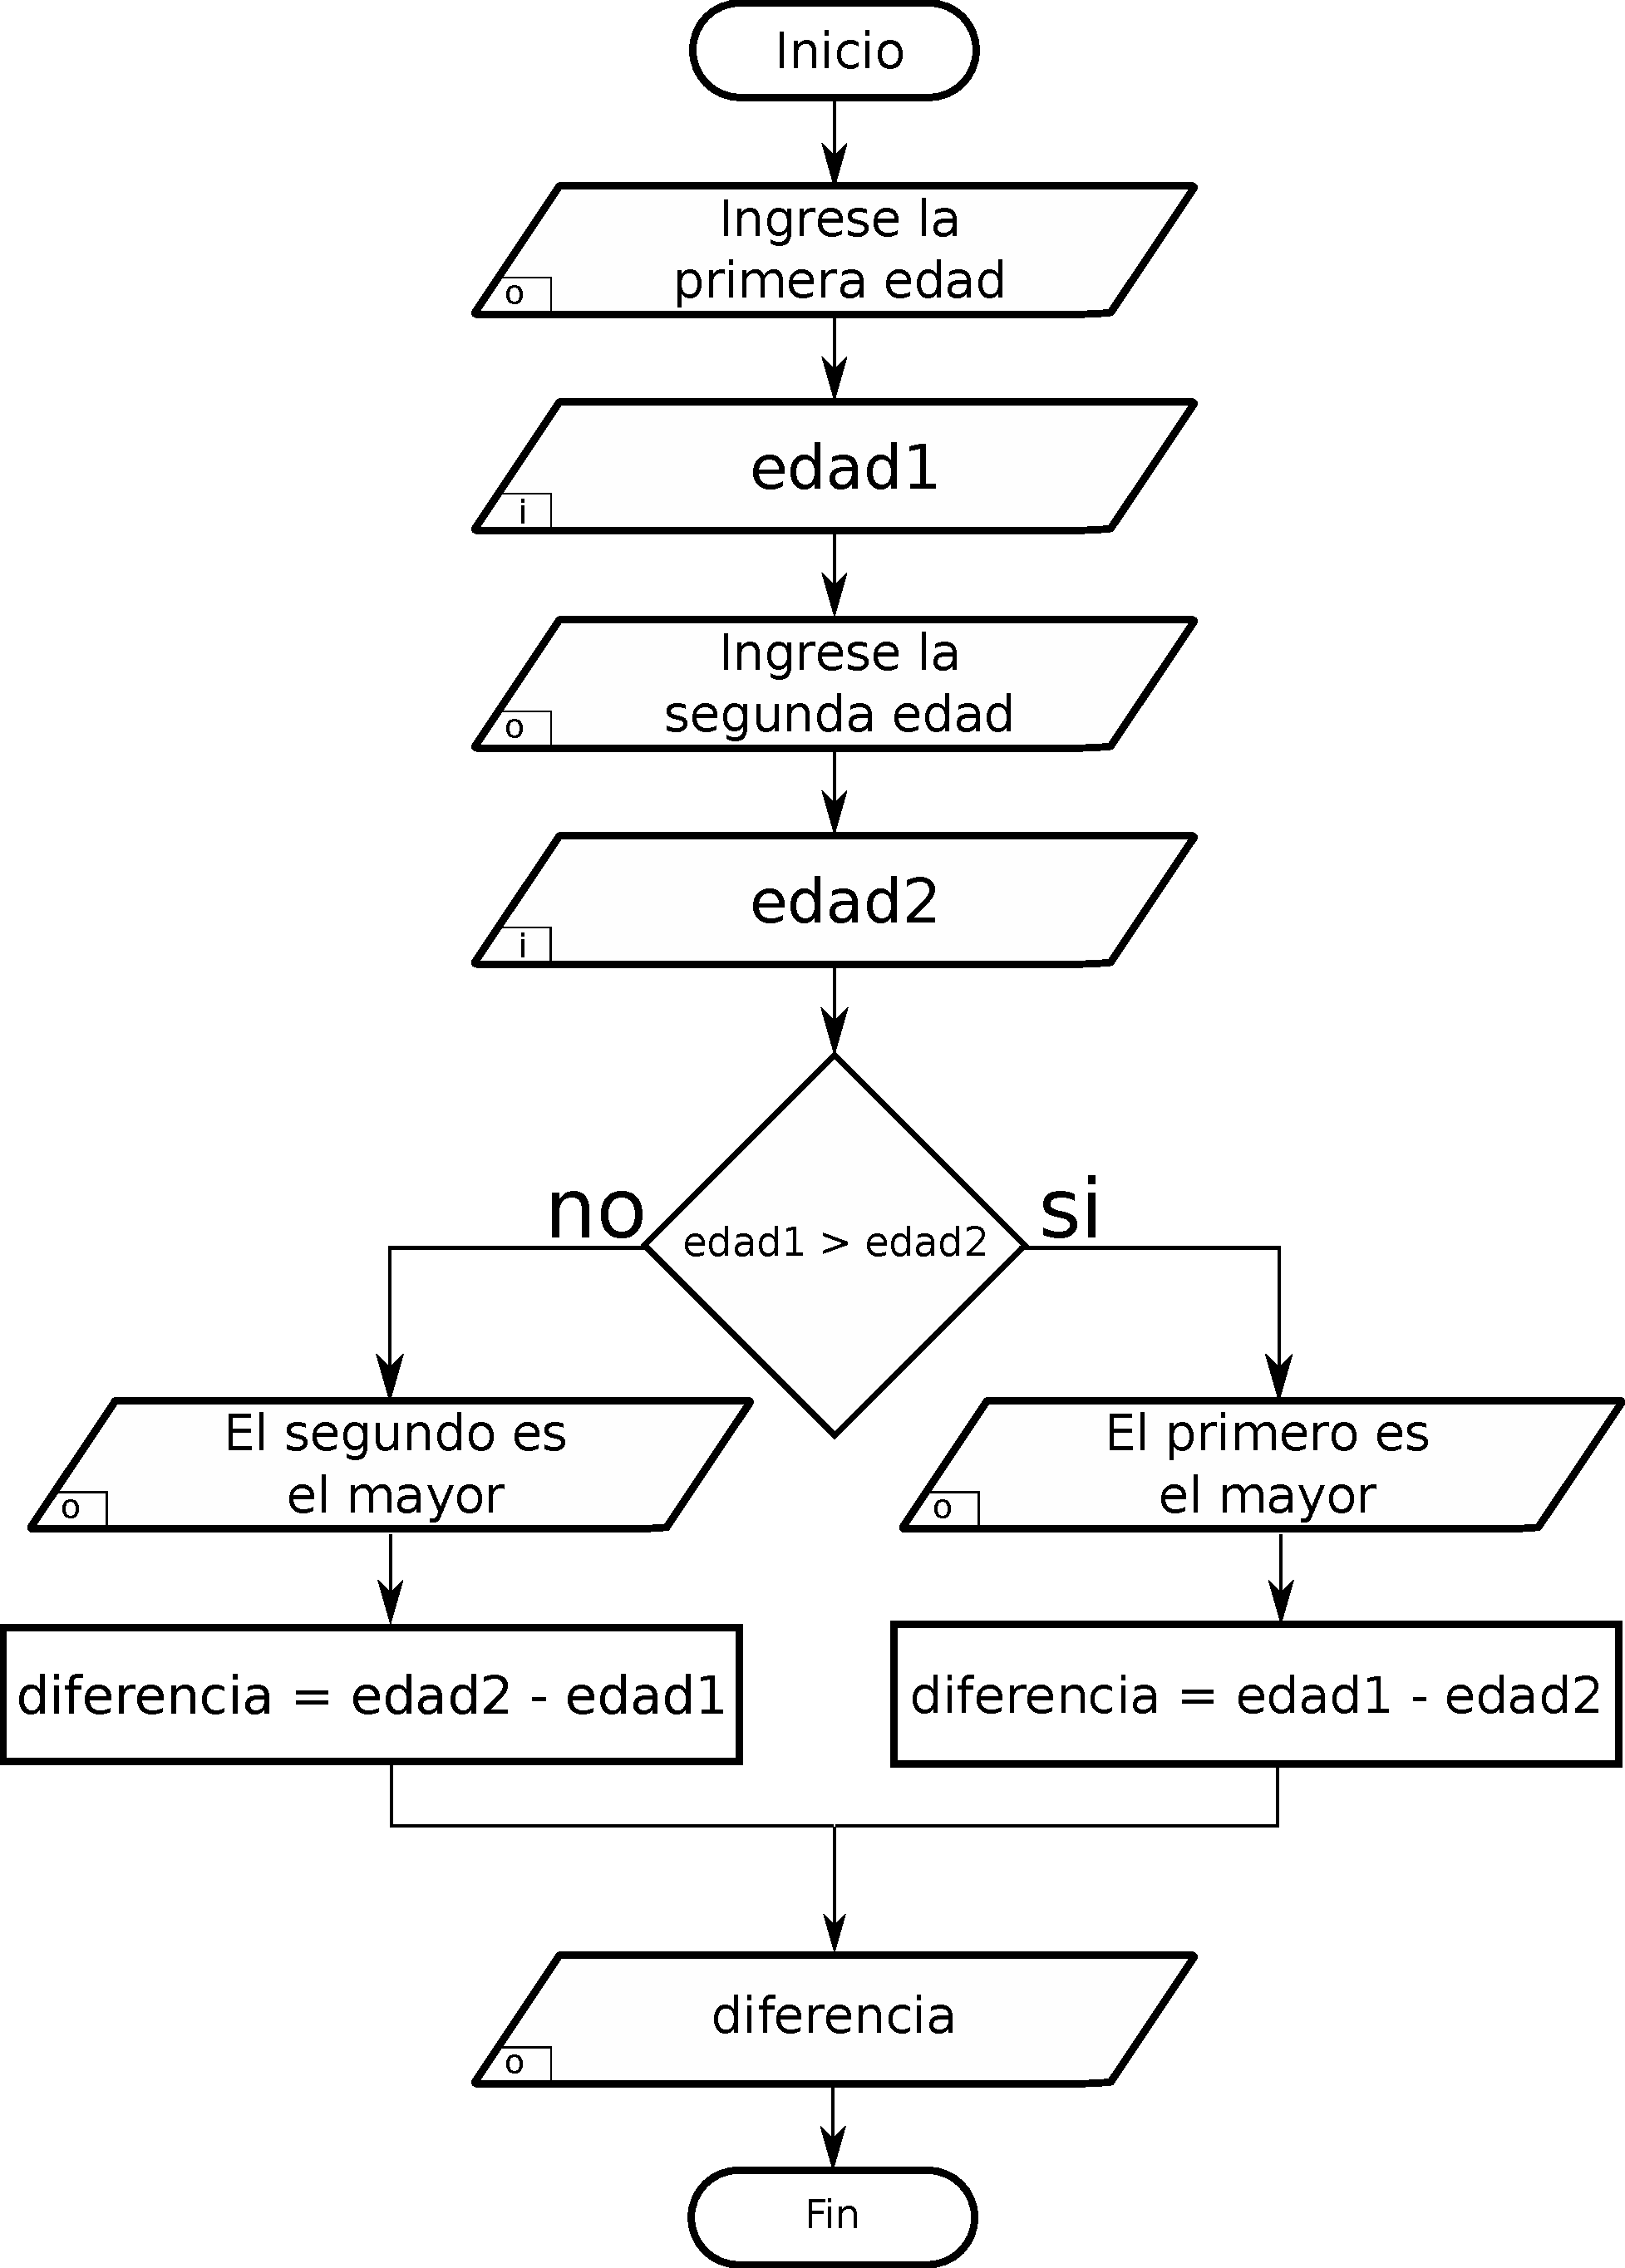
\includegraphics[height=150mm]{./img/ejercicio_2.pdf} 
\end{figure}

\pagebreak

\subsubsection{Ejercicio}
Escribir un algoritmo que imprima los números enteros desde el 0 hasta $N$. Donde el número $N$ es ingresado por el usuario.

\begin{lstlisting}[style=pseudocodigo]
imprimir: Ingrese N
leer: cantidad
para contador desde 0 hasta cantidad hacer
imprimir: contador
fin para
\end{lstlisting}

\begin{figure}[h!]
  \centering
  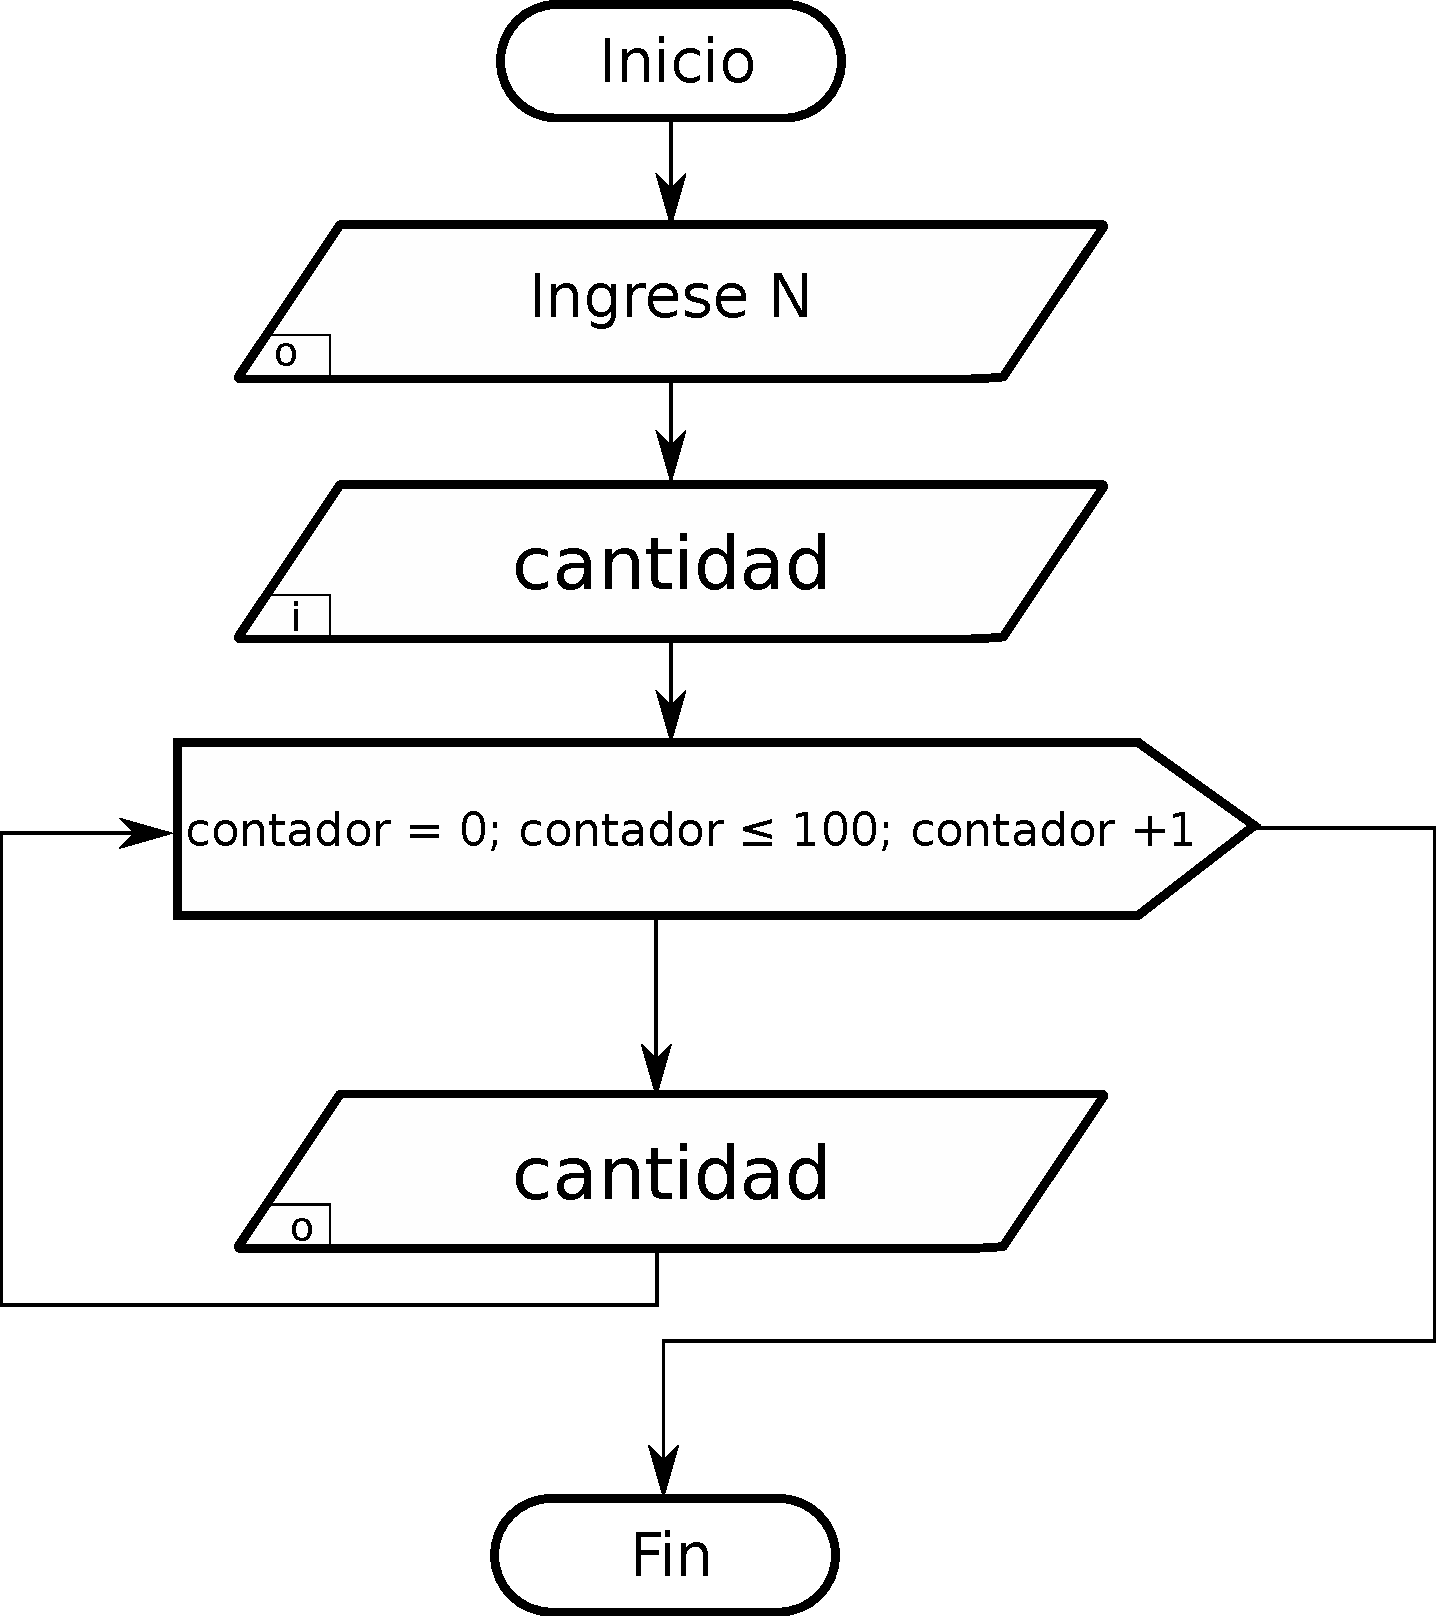
\includegraphics[height=110mm]{./img/ejercicio_3.pdf} 
  \caption{ejercicio 2 versión con bloque \textbf{para}}
\end{figure}

\pagebreak
\subsubsection{Preguntas:}
Completar los espacios en blanco:\\
\begin{enumerate}[a)]
  \item Todos los programas pueden ser escritos en términos de 3 secuencias de control:\underspace,\underspace,\underspace.
  \item La secuencia de control \underspace es utilizada para ejecutar una acción cuando es verdadera y otra acción cuando es falsa.
  \item La secuencia \underspace especifica que una o varias sentencias se ejecutarán repetidamente, mientras la condición sea verdadera.
\end{enumerate}


\pagebreak
% \subsubsection*{Selección}
\subsubsection{Ejercicio}
Escribir un algoritmo para calcular la distancia recorrida (m) por un móvil que se desplaza con velocidad constante (m/s) durante un tiempo (s). 
La velocidad y el tiempo serán ingresadas por el usuario.

\subsubsection{Ejercicio}
Escribir un algoritmo para obtener el promedio simple de un estudiante a partir de las tres notas parciales.
Las notas serán introducidas una a una por el usuario.

\subsubsection{Ejercicio}
En un local se hace un descuento del \%20 cuando la compra supera los \$ 1000. Escribir un algoritmo que calcule el precio a pagar por el cliente
teniendo como dato el valor de la compra.

\subsubsection{Ejercicio}
Escribir un algoritmo que determine si un número $n$ tiene tres cifras. El usuario debe ingresar el número $n$.

\subsubsection{Ejercicio 7}
Escribir un algoritmo que solicite ingresar dos números $n1$ y $n2$. Si el primero es mayor que el segundo mostrar la suma de ambos, por otro lado si el segundo es mayor al primero, mostrar el producto entre los números. En caso de que sean iguales imprimir ``Los números son iguales''.

% \subsubsection{Repetición}
\subsubsection{Ejercicio 8}
Escribir un programa que calcule la potencia $x={num1}^{num2}$, donde $num1$ y $num2$ son números enteros positivos ingresados por el usuario.

\subsubsection{Ejercicio 9}
Escribir un programa que calcule la suma de los primeros \textbf{n} números. El número \textbf{n} es un entero positivo, ingresado por el usuario.

\subsubsection{Ejercicio 10}
Escribir un algoritmo que imprima los número impares desde 0 hasta $N$. Donde $N$ es ingresado por el usuario.

\subsubsection{Ejercicio 11}
Escribir un algoritmo que determine la temperatura promedio de $N$ mediciones de temperatura. El usuario debe ingresar la cantidad $N$ y las $N$ mediciones. 

\subsubsection{Ejercicio 12}
Escribir un algoritmo que determine el mayor de 10 números ingresados. El usuario debe ingresar cada uno de los 10 números.

\subsubsection{Ejercicio 13}
Escribir un algoritmo que determine el mayor de $N$ números positivos ingresados. El usuario debe ingresar cada uno de los $N$ números. Para terminar se debe ingresar un -1.

\subsubsection{Ejercicio 14}
Escribir un algoritmo que solicite ingresar $N$ calificaciones de alumnos y determine la cantidad de aprobados, desaprobados y promocionados. 
El usuario debe ingresar el número $N$ y las $N$ calificaciones.

\underline{Según:}
\begin{itemize}
  \item Desaprobado: nota menor a 6
  \item Aprobado: nota mayor o igual a 6
  \item Promocionado: nota mayor o igual a 8
\end{itemize}

\subsubsection{Ejercicio 15}
Escribir de cuatro formas diferentes, sentencias en C que incrementen en 1 una variable \texttt{X}.


  \section{Control de flujo en lenguaje~C.}
\setcounter{subsection}{4}

\subsection{if, if else}

\subsubsection{Solución 0} 

\lstset{inputencoding=utf8/latin1}
\lstinputlisting[style=customc]{code/ejercicio0.c}
{\small
  \lstset{inputencoding=utf8/latin1}
  \lstinputlisting[backgroundcolor = \color{lightgray}]{code/ejercicio0_salida.mn}
}

\subsubsection{Ejercicio 1} 
Realizar un programa que determine el mayor entre dos números ingresados por el usuario
{\small
  \lstset{inputencoding=utf8/latin1}
  \lstinputlisting[backgroundcolor = \color{lightgray}]{code/ejercicio1_salida.mn}
}

\subsubsection{Ejercicio 2} 
Realizar un programa que determine el mayor entre tres números ingresados por el usuario. En caso de que trés o dos números sean iguales y los mayores, es indistinta la elección del mayor.
{\small
  \lstset{inputencoding=utf8/latin1}
  \lstinputlisting[backgroundcolor = \color{lightgray}]{code/ejercicio2_salida.mn}
}

\subsubsection{Ejercicio 3} 
Realizar un programa que controle el encendido de un ventilador en base a la temperatura de encendido y la temperatura ambiente proporcionada por el usuario. Se debe imprimir en pantalla el estado del ventilador luego de ingresar los datos.
{\small
  \lstset{inputencoding=utf8/latin1}
  \lstinputlisting[backgroundcolor = \color{lightgray}]{code/ejercicio3_salida.mn}
}

\subsubsection{Ejercicio 4} 
Realizar un programa que solicite ingresar las notas de dos parciales. Si desaprobó un parcial el programa debe solicitar ingresar la nota del recuperatorio. En base a las notas obtenidas calcular el promedio y determinar la condición académica (Promoción mayor 8, desaprobado menor a 6, lo demás aprobado). Solo se permite recuperar un solo parcial. La nota del recuperatorio se promedia con las notas del parcial y está permitido promocionar si recuperó.
{\small
  \lstset{inputencoding=utf8/latin1}
  \lstinputlisting[backgroundcolor = \color{lightgray}]{code/ejercicio4_salida.mn}
}

\subsubsection{Ejercicio 5} 
Realizar un programa que dada la duracion en minutos de una llamada, permita calcular el costo,considerando:\\
-Hasta tres minutos el costo es 0.50 por minuto
-Por encima de tres minutos es 1.5 fijo más 0.2 por cada minuto adicional a los tres primeros
{\small
  \lstset{inputencoding=utf8/latin1}
  \lstinputlisting[backgroundcolor = \color{lightgray}]{code/ejercicio5_salida.mn}
}



\subsection*{Operadores II, \&\&} 
Realizar un programa que determine si 3 números ingresados son distintos entre ellos.
\subsubsection{Solución 0} 

\lstset{inputencoding=utf8/latin1}
\lstinputlisting[style=customc]{code/ejercicio0.c}
{\small
  \lstset{inputencoding=utf8/latin1}
  % \lstinputlisting[backgroundcolor = \color{lightgray}]{code/ejercicio0_salida.mn}
}

\subsubsection{Ejercicio 1} 
Realizar un programa que determine si un número ingresado por el usuario está en el rango 10-100. En caso de no estar en el rango, el programa de be informarlo y terminar. Si el número está dentro del rango, el programa debe determinar si el número es par.
{\small
  \lstset{inputencoding=utf8/latin1}
  \lstinputlisting[backgroundcolor = \color{lightgray}]{code/ejercicio1_operadores_salida.mn}
}

\subsubsection{Ejercicio 2} 
Escribir un programa que determine el mayor de 3 números ingresados. Si los números son iguales, se debe imprimir un mensaje que lo indique.
{\small
  \lstset{inputencoding=utf8/latin1}
  \lstinputlisting[backgroundcolor = \color{lightgray}]{code/ejercicio2_operadores_salida.mn}
}

\subsubsection{Ejercicio 3} 
Realizar un programa que solicite ingresar el valor nominal de resistencia (en ohms) y la tolerancia (valor entero en porcentaje). Una vez cargados estos valores, el programa debe solicitar al usuario que ingrese un valor de resistencia real y determine si la misma está dentro de los márgenes de tolerancia. 
{\small
  \lstset{inputencoding=utf8/latin1}
  \lstinputlisting[backgroundcolor = \color{lightgray}]{code/ejercicio3_operadores_salida.mn}
}

\subsubsection{Ejercicio 4} 
Realizar un programa que determine si el caracter ingresado es un número o una letra. Ayuda: buscar ``tabla ASCII''.
{\small
  \lstset{inputencoding=utf8/latin1}
  \lstinputlisting[backgroundcolor = \color{lightgray}]{code/ejercicio4_operadores_salida.mn}
}

\subsubsection{Ejercicio 5} 
Modificar el programa anterior para que ahora solicite ingresar el color de las bandas de colores y la medición real de la resisitencia. Con estos valores el programa debe determinar si se encuentra dentro de los valores de tolerancia o no. Considerar el caso de resistencias de 4 bandas de colores, donde las primeras tres indican el valor de resistencia y el cuarto la tolerancia (dorado $ \pm 5 $, plateado $\pm 10$, rojo $\pm 2$ y marrón $\pm 1$. Los colores de las bandas serán ingresados en forma de caracteres. Cada caracter representa un color.
\begin{itemize}
  \item \textbf{N}egro
  \item \textbf{M}arrón
  \item \textbf{R}ojo
  \item naran\textbf{J}a
  \item \textbf{A}marillo
  \item \textbf{V}erde
  \item a\textbf{Z}ul
  \item vio\textbf{L}eta
  \item \textbf{G}ris
  \item \textbf{B}lanco
  \item \textbf{D}orado
  \item \textbf{P}lateado
  \end{itemize}
{\small
  \lstset{inputencoding=utf8/latin1}
  \lstinputlisting[backgroundcolor = \color{lightgray}]{code/ejercicio5_operadores_salida.mn}
}

\subsection*{Estructura repetitiva for}
Todos los ejercicios deben utilizar al menos una estructura \textbf{for}.
Algunos ejercicios pueden requerir utilizar estructuras de condición.

\subsubsection{Ejercicio 0} 
Realizar un programa que imprima los números desde el 5 hasta el 0 y luego vuelva hasta el 5 como en el siguiente ejemplo (se debe utilizar al menos una estructura for)

\subsubsection{Solución 0} 

\lstset{inputencoding=utf8/latin1}
\lstinputlisting[style=customc]{code/ejercicio0.c}
{\small
  \lstset{inputencoding=utf8/latin1}
  \lstinputlisting[backgroundcolor = \color{lightgray}]{code/ejercicio0_salida.mn}
}
\subsubsection{Solución 0 (con un solo for)} 
\lstinputlisting[style=customc]{code/ejercicio0_un.c}
{\small
  \lstset{inputencoding=utf8/latin1}
  \lstinputlisting[backgroundcolor = \color{lightgray}]{code/ejercicio0_salida.mn}
}

\subsubsection{Preguntas}
\begin{itemize}
  \item La iteración controlada por contador también se conoce como iteración \underspace porque se sabe de antemano cuántas veces se ejecutará el bucle.
  \item La iteración controlada por centinela también se conoce como iteración \underspace porque no se sabe de antemano cuántas veces se ejecutará el bucle.
  \item En la iteración controlada por contador, se usa un(una)\underspace  para contar el número de veces que se debe repetir un grupo de instrucciones.
\end{itemize}

\subsubsection{Analizar código}
Encontrar el error en las siguientes códigos:
\begin{enumerate}
  \item .
  \lstinputlisting[style=customc]{code/ejercicio_rep_a.c}
  \item .
  \lstinputlisting[style=customc]{code/ejercicio_rep_b.c}
\end{enumerate}

\subsubsection{Ejercicio 1} 
Modificar el programa anterior para que imprima la progresión de números partiendo de un número $n$ positivo ingresado por el usuario. 
{\small
  \lstset{inputencoding=utf8/latin1}
  \lstinputlisting[backgroundcolor = \color{lightgray}]{code/ejercicio1_rep_salida.mn}
}

\subsubsection{Ejercicio 2} 
Realizar un programa que utilice una entructura \textbf{for} e impmrima la siguiente salida:
{\small
  \lstset{inputencoding=utf8/latin1}
  \lstinputlisting[backgroundcolor = \color{lightgray}]{code/ejercicio2_rep_salida.mn}
}

\subsubsection{Ejercicio 3} 
Realizar un programa que utilice una entructura \textbf{for} e impmrima la siguiente tabla:
{\small
  \lstset{inputencoding=utf8/latin1}
  \lstinputlisting[backgroundcolor = \color{lightgray}]{code/ejercicio3_rep_salida.mn}
}

\subsubsection{Ejercicio 4} 
Realizar un programa que utilice dos entructuras \textbf{for} para imprimir una matriz, donde la cantidad de filas y columnas son ingresados por el usuario como la siguiente:
{\small
  \lstset{inputencoding=utf8/latin1}
  \lstinputlisting[backgroundcolor = \color{lightgray}]{code/ejercicio4_rep_salida.mn}
}

\subsubsection{Ejercicio 5} 
Escribir un programa que imprima todos los números enteros pares entre el 0 y $n$, donde $n$ es un número entero ingresado por el usuario.
{\small
  \lstset{inputencoding=utf8/latin1}
  \lstinputlisting[backgroundcolor = \color{lightgray}]{code/ejercicio5_rep_salida.mn}
}

\subsubsection{Ejercicio 6} 
Escribir un programa que determine el mayor de 10 números enteros ingresados por el usuario.
{\small
  \lstset{inputencoding=utf8/latin1}
  \lstinputlisting[backgroundcolor = \color{lightgray}]{code/ejercicio6_rep_salida.mn}
}

\subsubsection{Ejercicio 7} 
Modificar el programa del ejercicio anterior para que determine también el mínimo número ingresado.
{\small
  \lstset{inputencoding=utf8/latin1}
  \lstinputlisting[backgroundcolor = \color{lightgray}]{code/ejercicio7_rep_salida.mn}
}

\subsubsection{Ejercicio 8} 
Realizar un programa que calcule la tabla de multiplicar de un número $n$ ingresado por el usuario.
{\small
  \lstset{inputencoding=utf8/latin1}
  \lstinputlisting[backgroundcolor = \color{lightgray}]{code/ejercicio8_rep_salida.mn}
}

\subsubsection{Ejercicio 9} 
Realizar un programa que calcule el factorial de un número $n$ ingresado por el usuario. Donde $0<n<10$.
{\small
  \lstset{inputencoding=utf8/latin1}
  \lstinputlisting[backgroundcolor = \color{lightgray}]{code/ejercicio9_rep_salida.mn}
}

\subsubsection{Ejercicio 10} 
Realizar un programa que calcule la potencia $m$ de número $n$, donde $m$ y $n$ son ingresado por el usuario. Operación: $n^m$.
{\small
  \lstset{inputencoding=utf8/latin1}
  \lstinputlisting[backgroundcolor = \color{lightgray}]{code/ejercicio10_rep_salida.mn}
}

\subsection*{Estructuras repetitivas while y do..while}
Todos los ejercicios deben utilizar al menos una estructura \textbf{for}.
Repetir ahora utilizando estructura \textbf{while} y \textbf{do..while}.



  \section{Arreglos en lenguaje C.}

\subsection*{Arreglos unidimensionales}
\setcounter{subsection}{6}

Los ejercicios de ésta guía utilizan \texttt{arreglos}, algún tipo de estructura repetitiva ( \textbf{for}, \textbf{while} o \textbf{do\dots while})
y estructuras de contról \textbf{if\dots else}

\subsubsection{Ejercicio 1} 
Completar el siguiente programa, para que solicite al usuario ingresar 10 números enteros, los almacene en un arreglo. Luego, se debe recorrer el arreglo convirtiendo los números negativos en positivos. Por último mostrar en pantalla el arreglo.
\lstset{inputencoding=utf8/latin1}
\lstinputlisting[style=customc]{code/ejercicio1_completar.c}
{\small
  \lstset{inputencoding=utf8/latin1}
  \lstinputlisting[backgroundcolor = \color{lightgray}]{code/ejercicio1_arreglo_uni_salida.mn}
}

\subsubsection{Ejercicio 2} 
Escribir un programa que solicite al usuario ingresar $N$ elementos de un arreglos. Luego recorrer el arreglo, buscar el mayor elemento e imprimirlo.
{\small
  \lstset{inputencoding=utf8/latin1}
  \lstinputlisting[backgroundcolor = \color{lightgray}]{code/ejercicio2_arreglo_uni_salida.mn}
}

\subsubsection{Ejercicio 3} 
Escribir un programa que solicite ingresar $N$ elementos de un arreglo. Luego, en otro arreglo, almacenar el valor acumulado del primer arreglo. Por ejemplo: el elemento del segundo arreglo b[0] será a[0], el elemento b[1] contendrá la suma a[0]+a[1], el elemento b[3] contedrá la suma a[0]+a[1]+a[2]+a[3]
{\small
  \lstset{inputencoding=utf8/latin1}
  \lstinputlisting[backgroundcolor = \color{lightgray}]{code/ejercicio3_arreglo_uni_salida.mn}
}

\subsubsection{Ejercicio 4} 
Realizar un programa que solicite al usuario ingresar $N$ elementos de un arreglo. Los valores a ingresar tienen que estar en el rango de (1-100), en caso de ingresar un valor fuera del rango, se debe volver a pedir el valor.
{\small
  \lstset{inputencoding=utf8/latin1}
  \lstinputlisting[backgroundcolor = \color{lightgray}]{code/ejercicio4_arreglo_uni_salida.mn}
}
\subsubsection{Ejercicio 5} 
Realizar un programa que solicite ingresar $N$ componentes de dos vectores \textbf{a} y \textbf{b}. Luego calcular el producto punto entre los mismos.
Recordar que el producto punto se puede expresar como:
$$\overrightarrow{a}\cdot \overrightarrow{b} = a_1\cdot b_1 + a_2\cdot b_2 +\dots + a_N\cdot b_N$$
{\small
  \lstset{inputencoding=utf8/latin1}
  \lstinputlisting[backgroundcolor = \color{lightgray}]{code/ejercicio5_arreglo_uni_salida.mn}
}

\subsubsection{Preguntas} 
\begin{itemize}
  \item El número por el cual se refiere a un elemento particular de un arreglo se llama:
  \item El primer elemento de un arreglo es el número[(completar aquí)].
\end{itemize}

\subsubsection{Indicar verdadero o falso:}
\begin{itemize}
  \item Un arreglo puede tener elementos de diferentes tipos.
  \item El índice de un arreglo puede ser de tipo \texttt{double}
  \item En una inicialización de un arreglo, si hay una cantidad menor de elementos que el tamaño del arreglo, C automáticamente inicializa los elementos restantes con el último elemento de la lista de inicialización.
  \item Es un error si en la inicialización de un arreglo hay mas elementos que el tamaño del arreglo.
  \item Si hay menos elementos en la lista de inicialización de un arreglo que el tamaño del arreglo, los elementos restantes son inicializados con basura.
\end{itemize}

\subsection*{Arreglos Bidimensionales} 

\subsubsection{Ejercicio 1} 
Escribir un programa quje solicite al usuario ingresar un arreglo de dos dimensiones de \textit{NxM}. \textit{N} y \textit{M} son directivas de preprocesador. Al finalizar, el programa debe imprimir la matriz.

\subsubsection{Ejercicio 2} 
Escribir un programa que solicite ingresar al usuario los elementos de un arreglo bidimensional de \textbf{n} filas por  \textbf{m} columnas. Los valores de \textbf{n} y \textbf{m} son ingresados por el usuario, los mismos deben ser menores que N y M (directivas de preprocesador) y mayores que 0. Imprimir el arreglo al finalizar.

\subsubsection{Ejercicio 3} 
Escribir un programa quje solicite al usuario ingresar un arreglo de dos dimensiones de \textit{NxM}. \textit{N} y \textit{M} son directivas de preprocesador. Luego se deben copiar los elementos del arreglo se deben copiar a otro arreglo, de tal manera de obtener la matriz transpuesta.
Al finalizar, el programa debe imprimir las dos matrices.

\subsubsection{Ejercicio 4} 
Modificar el programa anterior para obtener el producto de una matriz por su transpuesta. El producto entre las matrices $A*B$ es una mtriz C donde:

$$C_{ij}=\sum_{k=1}^{m}{A_{ik}B_{kj}} $$



  \section{Funciones en lenguaje C.}
\setcounter{subsection}{7}

\subsection*{Funciones $1^{era}$ Parte} 

\subsubsection{Ejercicio 1} 
Completar el siguiente programa:

\lstset{inputencoding=utf8/latin1}
\lstinputlisting[style=customc]{code/ejercicio1_fun_completar_guia.c}
{\small
  \lstset{inputencoding=utf8/latin1}
  \lstinputlisting[backgroundcolor = \color{lightgray}]{code/ejercicio1_completar_salida.mn}
}

\subsubsection{Ejercicio 2} 
Completar el siguiente programa:
\lstset{inputencoding=utf8/latin1}
\lstinputlisting[style=customc]{code/ejercicio2_completar_guia.c}
Para obtener la siguiente salida:
{\small
  \lstset{inputencoding=utf8/latin1}
  \lstinputlisting[backgroundcolor = \color{lightgray}]{code/ejercicio2_completar_salida.mn}
}

\subsubsection{Ejercicio 3} 
Completar el siguiente programa:
\lstset{inputencoding=utf8/latin1}
\lstinputlisting[style=customc]{code/ejercicio3_completar_guia.c}
Para obtener la siguiente salida:
{\small
  \lstset{inputencoding=utf8/latin1}
  \lstinputlisting[backgroundcolor = \color{lightgray}]{code/ejercicio3_completar_salida.mn}
}

\subsubsection{Ejercicio 4} 
Completar el siguiente programa:
\lstset{inputencoding=utf8/latin1}
\lstinputlisting[style=customc]{code/ejercicio4_completar_guia.c}
Para obtener la siguiente salida:
{\small
  \lstset{inputencoding=utf8/latin1}
  \lstinputlisting[backgroundcolor = \color{lightgray}]{code/ejercicio4_completar_salida.mn}
}

\subsubsection{Ejercicio 5}
Completar el siguiente programa:
\lstset{inputencoding=utf8/latin1}
\lstinputlisting[style=customc]{code/ejercicio5_completar_guia.c}
Para obtener la siguiente salida:
{\small
  \lstset{inputencoding=utf8/latin1}
  \lstinputlisting[backgroundcolor = \color{lightgray}]{code/ejercicio5_completar_salida.mn}
}


\subsubsection{Ejercicio 6} 
Completar el siguiente programa:
\lstset{inputencoding=utf8/latin1}
\lstinputlisting[style=customc]{code/ejercicio6_completar_guia.c}
Para obtener la siguiente salida:
{\small
  \lstset{inputencoding=utf8/latin1}
  \lstinputlisting[backgroundcolor = \color{lightgray}]{code/ejercicio6_completar_salida.mn}
}

\subsubsection{Ejercicio 7} 
Completar el siguiente programa:
\lstset{inputencoding=utf8/latin1}
\lstinputlisting[style=customc]{code/ejercicio7_completar_guia.c}
Para obtener la siguiente salida:
{\small
  \lstset{inputencoding=utf8/latin1}
  \lstinputlisting[backgroundcolor = \color{lightgray}]{code/ejercicio7_completar_salida.mn}
}

\subsubsection{Ejercicio 8} 
Crear los prototipos para las diferentes funciones que resuelvan:
\begin{itemize}
  \item Función \textbf{hipotenusa}, toma dos argumentos float de doble precisión, \textbf{lado1} y \textbf{lado2}. Devuelve el resultado en float de doble precisión.
  \item Función \textbf{menor}, toma tres enteros, \textbf{x}, \textbf{y}, \textbf{z}. Devuelve un entero.
  \item Función \textbf{intToFloat}, que toma un argumento entero llamado \textbf{numero}, y devuelve el resultado en float.
\end{itemize}


\subsection*{Funciones $2^{da}$ Parte} 

\subsubsection{Ejercicio 1} 
Implementar la función \texttt{fibonacci} en forma recursiva.

\lstset{inputencoding=utf8/latin1}
\lstinputlisting[style=customc]{code/ejercicio1_fun2_completar_guia.c}

\subsubsection{Ejercicio 2} 
El rompecabezas de la Torre de Hanoi fue inventado por el matemático francés Edouard Lucas en 1883. Se inspiró en una leyenda acerca de un templo hindú donde el rompecabezas fue presentado a los jóvenes sacerdotes. Al principio de los tiempos, a los sacerdotes se les dieron tres postes y una pila de 64 discos de oro, cada disco un poco más pequeño que el de debajo. 

Su misión era transferir los 64 discos de uno de los tres postes a otro, con dos limitaciones importantes. Sólo podían mover un disco a la vez, y nunca podían colocar un disco más grande encima de uno más pequeño. Los sacerdotes trabajaban muy eficientemente, día y noche, moviendo un disco cada segundo. Cuando terminaran su trabajo, dice la leyenda, el templo se desmenuzaría en polvo y el mundo se desvanecería.

En la Figura  Se puede ver la representación gráfica del juego.

% \begin{figure}[h!]
% \centering
% \includegraphics[width=\textwidth]{img/hanoi.eps}
% \caption{Torres de Hanoi\\ Fuente: Deitel\&Deitel}
% \label{fig:hanoi}
% \end{figure}
Supongamos que los sacerdotes intentan mover los discos de la clavija 1 a la clavija 3. Deseamos desarrollar un algoritmo que imprima la secuencia precisa de transferencias de clavija de disco a disco.
Si tuviéramos que abordar este problema con métodos convencionales, nos encontraríamos rápidamente anudados en la gestión de los discos. En cambio, si atacamos el problema con la recursión en mente, inmediatamente se vuelve manejable. Mover n discos se puede ver en términos de mover solo n - 1 discos (y, por lo tanto, la recursividad) de la siguiente manera:
\begin{enumerate}
  \item Mueva n - 1 discos de la clavija 1 a la clavija 2, utilizando la clavija 3 como área de retención temporal.
  \item Mueva el último disco (el más grande) de la clavija 1 a la clavija 3.
  \item Mueva los discos n - 1 de la clavija 2 a la clavija 3, utilizando la clavija 1 como área de retención temporal.
\end{enumerate}
El proceso finaliza cuando la última tarea implica mover n = 1 disco, es decir, el caso base. Esto se logra moviendo trivialmente el disco sin la necesidad de un área de retención temporal.
Escribe un programa para resolver el problema de Towers of Hanoi. Use una función recursiva con cuatro parámetros:
\begin{enumerate}
  \item El número de discos a mover
  \item La clavija en la que se enroscan estos discos inicialmente
  \item La clavija a la que se debe mover esta pila de discos
  \item La clavija que se utilizará como área de retención temporal.
\end{enumerate}
Su programa debe imprimir las instrucciones precisas que necesitará para mover los discos desde la clavija de inicio a la clavija de destino. Por ejemplo, para mover una pila de tres discos de la clavija 1 a la clavija 3, su programa debe imprimir la siguiente serie de movimientos:

{\scriptsize
  \lstset{inputencoding=utf8/latin1}
  \lstinputlisting[backgroundcolor = \color{lightgray}]{code/hanoi_salida.mn}
}

\pagebreak
\subsubsection{Ejercicio 3} 
Modificar el siguiente programa, para que los valores del arreglo sean ingresados con la función \textbf{carga}.
\lstset{inputencoding=utf8/latin1}
\lstinputlisting[style=customc]{code/ejercicio1_fun2_completar.c}
Prototipo de la función \textbf{carga}
\lstset{inputencoding=utf8/latin1}
\lstinputlisting[style=customc]{code/carga.c}

\subsubsection{Ejercicio 4} 
Modificar el programa anterior para que la impresión del arreglo se realice con la función con prototipo:
\lstset{inputencoding=utf8/latin1}
\lstinputlisting[style=customc]{code/imprime.c}

\subsubsection{Ejercicio 5} 
Modificar el programa anterior para que el arreglo ingresado se ordene de mayor a menor con la función con prototipo:
\lstset{inputencoding=utf8/latin1}
\lstinputlisting[style=customc]{code/ordenar.c}

\subsubsection{Ejercicio 6} 
Modificar el programa del Ejercicio 4, para que se imprima la cantidad de números primos en el arreglo. Utilizar los prototipos:
\lstset{inputencoding=utf8/latin1}
\lstinputlisting[style=customc]{code/primos.c}

\subsubsection{Ejercicio 7} 
Modificar el programa del Ejercicio 4, para que se imprima el mayor y el menor de los números en el arreglo, utilizando los prototipos:
\lstset{inputencoding=utf8/latin1}
\lstinputlisting[style=customc]{code/mayor.c}




  \section{Punteros en lenguaje C.}
\setcounter{subsection}{8}

\subsection*{Paso de parámetros por referencia}
Se solicita un programa que cumpla con lo siguiente:
\begin{itemize}[a)]
  \item Requisito 1
    El usuario debe ingresar \textbf{N} valores en un arreglo unidimensional. Los valores ingresados solo pueden ser positivos (incluyendo el cero) menores que 100.

    Se debe realizar la validación en una función que reciba el parámetro por referencia.

  \item Requisito 2
    Una vez cargados los \textbf{N} valores se debe controlar que no haya números primos. Si existiesen deben ser incrementados en una unidad. Implementar esto en una función,
    que debe recibir el valor que debe ser chequeado por referencia.

  \item Requisito 3
    Debe ordenarse el arreglo de mayor a menor utilizando el método de la burbuja. Debe implementarse una función llamada \textit{swap}
    que reciba por referencia los dos elementos del arreglo que deben intercambiarse para lograr el ordenamiento.

  \item Requisito 4
    Debe imprimirse el arreglo antes y después del ordenamiento.


    \hspace{-5mm}El siguiente programa de ejemplo puede servir de ayuda:

    \lstset{inputencoding=utf8/latin1}
    \lstinputlisting[style=customc]{code/ejercicio_demo.c}
\end{itemize}


  \section{Estructuras y uniones en C. Campos de bit.}
\setcounter{subsection}{9}

\subsection*{Estructuras}
\subsubsection{Ejercicio 1}
Crear las estructuras según los siguientes requerimientos:
\begin{itemize}
  \item Una estructura \texttt{inventario} que contenga un arreglo de 30 char llamado \texttt{nombre}, un entero \texttt{numero\_parte}, flotante \texttt{precio}, y un entero \texttt{stock}
  \item  Una estrucura que contenga los siguientes arreglos: un arreglo de 20 elementos para el nombre de la calle \texttt{direccion}, un arreglo \texttt{ciudad} de 25 elementos para el nombre de la ciudad, un arreglo \texttt{codpost} de 6 elementos para el código postal.
\end{itemize}
Dentro de \texttt{main} se tienen inicializar las estructuras anteriores.

\subsubsection{Ejercicio 2} 
Dada la siguiente estructura:
\lstset{inputencoding=utf8/latin1}
\lstinputlisting[style=customc]{code/estructura.c}
Escribir un programa que cumpla con:
\begin{enumerate}[a)]
  \item Solicitar al usuario ingresar cada dato de la estructura y almacenarlo.
  \item Imprimir los datos cargados por el usuario.
\end{enumerate}

\subsubsection{Ejercicio 3} 
 Completar el siguiente programa para ingresar los miembros de cada elemento de tipo \texttt{alumno} en el arreglo \texttt{alumnos}.
\lstset{inputencoding=utf8/latin1}
\lstinputlisting[style=customc]{code/ejercicio3_estructuras.c}
El programa debe cumplir:
\begin{itemize}
  \item Se debe validar que el legajo y DNI sea un número positivo
  \item El usuario debe cargar las 3 notas. Luego con esta información, el programa calcula y almacena el promedio de cada alumno en el miembro \texttt{promedio}.
  \item El programa debe determinar el \texttt{estado} académico del alumno según:
    \begin{itemize}
      \item Promoción: promedio mayor o igual a 8.
      \item Regular: promedio maoyor o igual a 6 y menor que 8.
      \item Libre: promedio menor a 6.
    \end{itemize}
\end{itemize}

\subsection*{Uniones y Enumeraciones}

\subsubsection{Ejercicio 1} 
En los siguientes fragmentos de programa, determinar si son correctos o no. En caso de no serlo justificar.
\begin{enumerate}[a)]
  \item \_
  \lstset{inputencoding=utf8/latin1}
  \lstinputlisting[style=customc]{code/teo0.c}
  \item \_
  \lstset{inputencoding=utf8/latin1}
  \lstinputlisting[style=customc]{code/teo1.c}
  \item Suponga que estructura \texttt{carta} se ha definido con dos punteros para char (número y palo).
  %\lstset{inputencoding=utf8/latin1}
  %\lstinputlisting[style=customc]{teo3.c}
    Además, la variable c se ha definido para ser de tipo struct carta y la variable cPtr se ha definido para ser de tipo puntero a struct carta. 
    A la variable cPtr se le ha asignado la dirección de c.
  \lstset{inputencoding=utf8/latin1}
  \lstinputlisting[style=customc]{code/teo4.c}
\end{enumerate}
\subsubsection{Ejercicio 2} 
Indique si cada uno de los siguientes es verdadero o falso. Si es falso, explique por qué.
\begin{enumerate}[a)]
  \item Las estructuras pueden contener variables de un solo tipo de datos.
  \item Se pueden comparar dos uniones (usando ==) para determinar si son iguales.
  \item El nombre de la etiqueta de una estructura es opcional.
  \item Los miembros de diferentes estructuras deben tener nombres únicos.
  \item La palabra clave typedef se usa para definir nuevos tipos de datos.
  \item Las estructuras siempre se pasan a las funciones por referencia.
  \item Las estructuras no pueden compararse utilizando operadores == y! =.
\end{enumerate}

\subsubsection{Ejercicio 3} 
Escriba el código para lograr cada uno de los siguientes:
\begin{enumerate}[a)]
  \item Defina una estructura llamada parte que contenga la variable int sin signo partNumber y char array partName con valores que pueden tener hasta 25 caracteres (incluido el carácter nulo de terminación).
  \item Definir Parte como sinónimo de la parte de tipo estructura.
  \item Use Part para declarar que la variable a sea de tipo struct part, la matriz b [10] sea de tipo struct parte y la variable ptr para que sea de tipo puntero a struct part.
  \item Lea un número de parte y un nombre de parte del teclado en los miembros individuales de la variable a.
  \item Asigne los valores de miembro de la variable a al elemento 3 de la matriz b.
  \item Asigne la dirección de la matriz b a la variable de puntero ptr.
  \item Imprima los valores de miembros del elemento 3 de la matriz b usando la variable ptr y el operador de puntero de estructura para referirse a los miembros.
\end{enumerate}
\subsubsection{Ejercicio 4} 
Dada la estructura  \texttt{personaje\_t}, realizar un programa que solicite al usuario ingresar los datos necesarios para completar la estructura.
Los miembros \texttt{escudo} y \texttt{sales} deben ser inicializados en 0. 
El miembro \texttt{vida} en $150.0$.
El miembro \texttt{rango} se debe generar en forma aleatoria, con un valor entre $0$ y $100$.
\lstset{inputencoding=utf8/latin1}
\lstinputlisting[style=customc]{code/personaje.c}
El programa debe cargar los miembros mediante dos formas: la primera en forma directa con la variable \texttt{personaje}, y en forma indirecta mediante el puntero \texttt{pPersonaje} según la siguiente definición:

\lstset{inputencoding=utf8/latin1}
\lstinputlisting[style=customc]{code/sol_personaje_ej.c}
Acontinuación se adjunta un ejemplo de salida válido:
\lstset{inputencoding=utf8/latin1}
{\small
\lstinputlisting[backgroundcolor = \color{lightgray}]{code/sol_personaje_salida.mn}
}

\subsection*{Campos de bits}
\subsubsection*{Ejercicio 1} 
Dado el siguiente programa, implementar las funciones según las especificaciones indicadas en los comentarios.
El mazo de cartas debe ser inicializado de manera aleatoria, estando permitida la repetición de cartas.
\lstset{inputencoding=utf8/latin1}
\lstinputlisting[style=customc]{code/ejercicio1_campo.c}
A continuación se muestra un ejemplo de salida del programa:
\lstset{inputencoding=utf8/latin1}
{\small
\lstinputlisting[backgroundcolor = \color{lightgray}]{code/ejercicio1_campo_completo_salida.mn}
}




  \section{Manejo de archivos en C.}
\setcounter{subsection}{10}

\subsection*{Preguntas:}
\begin{itemize}[a)]
  \item Completar los espacios en blanco:\\
    \begin{enumerate}
      \item La función \underspace cierra un archivo.
      \item La función \underspace lee los datos de un archivo de manera similar a cómo scanf lee desde stdin.
      \item La función \underspace lee un caracter de un archivo especificado.
      \item La función \underspace reposiciona el puntero de posición del archivo a una ubicación específica en el archivo.
    \end{enumerate}
\end{itemize}
\subsubsection{Ejercicio 1}
Indique cuáles de los siguientes son verdaderos y cuáles son falsos.\\
Si es falso, explique por qué.
\begin{itemize}[a)]
  \item La función fscanf no se puede usar para leer datos de la entrada estándar.
  \item Debe usar explícitamente fopen para abrir la entrada estándar, la salida estándar y las secuencias de error estándar.
  \item Un programa debe llamar explícitamente a la función fclose para cerrar un archivo.
  \item Si el puntero de posición del archivo apunta a una ubicación en un archivo secuencial que no sea el comienzo del archivo, el archivo debe cerrarse y volverse a abrir para leerlo desde el principio del archivo.
  \item La función fprintf puede escribir en la salida estándar.
  \item Los datos en archivos de acceso secuencial siempre se actualizan sin sobrescribir otros datos.
  \item No es necesario buscar a través de todos los registros en un archivo de acceso aleatorio para encontrar un registro específico.
  \item Los registros en archivos de acceso aleatorio no tienen una longitud uniforme.
  \item La función fseek puede buscar solo en relación con el comienzo de un archivo.
\end{itemize}



\subsubsection*{Ejercicio 2} 
Encuentre el error en cada uno de los siguientes segmentos del programa y explique cómo corregirlo.
\begin{enumerate}[a)]
  \item El archivo al que hace referencia fPtr ("pagos.dat") no se ha abierto.
    \lstset{inputencoding=utf8/latin1}
    \lstinputlisting[style=customc]{code/ejercicio2a.c}
  \item \ \ \ 
    \lstinputlisting[style=customc]{code/ejercicio2b.c}
  \item La siguiente declaración debería leer un registro del archivo "pagos.dat". 
    El puntero de archivo payPtr se refiere a este archivo, y el puntero de archivo recPtr se refiere al archivo "recibir.dat"
    \lstinputlisting[style=customc]{code/ejercicio2c.c}
  \item El archivo "tools.dat" debe abrirse para agregar datos al archivo sin descartar los datos actuales.
    \lstinputlisting[style=customc]{code/ejercicio2d.c}
  \item El archivo "course.dat" debe abrirse para agregarlo sin modificar el contenido actual del archivo.
    \lstinputlisting[style=customc]{code/ejercicio2e.c}
\end{enumerate}





  \section{Uso del lenguaje C en aplicaciones de bajo nivel.}


\end{document}
